\documentclass[twoside]{book}

% Packages required by doxygen
\usepackage{fixltx2e}
\usepackage{calc}
\usepackage{doxygen}
\usepackage[export]{adjustbox} % also loads graphicx
\usepackage{graphicx}
\usepackage[utf8]{inputenc}
\usepackage{makeidx}
\usepackage{multicol}
\usepackage{multirow}
\PassOptionsToPackage{warn}{textcomp}
\usepackage{textcomp}
\usepackage[nointegrals]{wasysym}
\usepackage[table]{xcolor}

% Font selection
\usepackage[T1]{fontenc}
\usepackage[scaled=.90]{helvet}
\usepackage{courier}
\usepackage{amssymb}
\usepackage{sectsty}
\renewcommand{\familydefault}{\sfdefault}
\allsectionsfont{%
  \fontseries{bc}\selectfont%
  \color{darkgray}%
}
\renewcommand{\DoxyLabelFont}{%
  \fontseries{bc}\selectfont%
  \color{darkgray}%
}
\newcommand{\+}{\discretionary{\mbox{\scriptsize$\hookleftarrow$}}{}{}}

% Page & text layout
\usepackage{geometry}
\geometry{%
  a4paper,%
  top=2.5cm,%
  bottom=2.5cm,%
  left=2.5cm,%
  right=2.5cm%
}
\tolerance=750
\hfuzz=15pt
\hbadness=750
\setlength{\emergencystretch}{15pt}
\setlength{\parindent}{0cm}
\setlength{\parskip}{3ex plus 2ex minus 2ex}
\makeatletter
\renewcommand{\paragraph}{%
  \@startsection{paragraph}{4}{0ex}{-1.0ex}{1.0ex}{%
    \normalfont\normalsize\bfseries\SS@parafont%
  }%
}
\renewcommand{\subparagraph}{%
  \@startsection{subparagraph}{5}{0ex}{-1.0ex}{1.0ex}{%
    \normalfont\normalsize\bfseries\SS@subparafont%
  }%
}
\makeatother

% Headers & footers
\usepackage{fancyhdr}
\pagestyle{fancyplain}
\fancyhead[LE]{\fancyplain{}{\bfseries\thepage}}
\fancyhead[CE]{\fancyplain{}{}}
\fancyhead[RE]{\fancyplain{}{\bfseries\leftmark}}
\fancyhead[LO]{\fancyplain{}{\bfseries\rightmark}}
\fancyhead[CO]{\fancyplain{}{}}
\fancyhead[RO]{\fancyplain{}{\bfseries\thepage}}
\fancyfoot[LE]{\fancyplain{}{}}
\fancyfoot[CE]{\fancyplain{}{}}
\fancyfoot[RE]{\fancyplain{}{\bfseries\scriptsize Generated by Doxygen }}
\fancyfoot[LO]{\fancyplain{}{\bfseries\scriptsize Generated by Doxygen }}
\fancyfoot[CO]{\fancyplain{}{}}
\fancyfoot[RO]{\fancyplain{}{}}
\renewcommand{\footrulewidth}{0.4pt}
\renewcommand{\chaptermark}[1]{%
  \markboth{#1}{}%
}
\renewcommand{\sectionmark}[1]{%
  \markright{\thesection\ #1}%
}

% Indices & bibliography
\usepackage{natbib}
\usepackage[titles]{tocloft}
\setcounter{tocdepth}{3}
\setcounter{secnumdepth}{5}
\makeindex

% Hyperlinks (required, but should be loaded last)
\usepackage{ifpdf}
\ifpdf
  \usepackage[pdftex,pagebackref=true]{hyperref}
\else
  \usepackage[ps2pdf,pagebackref=true]{hyperref}
\fi
\hypersetup{%
  colorlinks=true,%
  linkcolor=blue,%
  citecolor=blue,%
  unicode%
}

% Custom commands
\newcommand{\clearemptydoublepage}{%
  \newpage{\pagestyle{empty}\cleardoublepage}%
}

\usepackage{caption}
\captionsetup{labelsep=space,justification=centering,font={bf},singlelinecheck=off,skip=4pt,position=top}

%===== C O N T E N T S =====

\begin{document}

% Titlepage & ToC
\hypersetup{pageanchor=false,
             bookmarksnumbered=true,
             pdfencoding=unicode
            }
\pagenumbering{alph}
\begin{titlepage}
\vspace*{7cm}
\begin{center}%
{\Large P\+PL Assignment }\\
\vspace*{1cm}
{\large Generated by Doxygen 1.8.13}\\
\end{center}
\end{titlepage}
\clearemptydoublepage
\pagenumbering{roman}
\tableofcontents
\clearemptydoublepage
\pagenumbering{arabic}
\hypersetup{pageanchor=true}

%--- Begin generated contents ---
\chapter{P\+PL assignment}
\label{index}\hypertarget{index}{}developed by Harpahul Singh Bhatia I\+I\+T2015082 
\chapter{ppl-\/assignment-\/kirihack13}
\label{md__r_e_a_d_m_e}
\Hypertarget{md__r_e_a_d_m_e}
ppl-\/assignment-\/kirihack13 created by Git\+Hub Classroom

tested on kali linux 2016.\+2 OS

build Q1 using \begin{DoxyVerb}  g++ boy.cpp girl.cpp make_rel.cpp rel.cpp Q1.cpp;
\end{DoxyVerb}


run using ./a.out

build Q2 using \begin{DoxyVerb}  g++ boy.cpp girl.cpp make_rel.cpp rel.cpp give_gift.cpp gift.cpp Q2.cpp;
\end{DoxyVerb}


run using ./a.out

input value of k for Q2 
\chapter{Hierarchical Index}
\section{Class Hierarchy}
This inheritance list is sorted roughly, but not completely, alphabetically\+:\begin{DoxyCompactList}
\item \contentsline{section}{boy}{\pageref{classboy}}{}
\item \contentsline{section}{breakup}{\pageref{classbreakup}}{}
\item \contentsline{section}{cp}{\pageref{structcp}}{}
\item \contentsline{section}{getgf}{\pageref{classgetgf}}{}
\item \contentsline{section}{gift}{\pageref{classgift}}{}
\item \contentsline{section}{girl}{\pageref{classgirl}}{}
\item \contentsline{section}{give\+\_\+gift}{\pageref{classgive__gift}}{}
\item \contentsline{section}{give\+\_\+gift\+\_\+\+Q5}{\pageref{classgive__gift___q5}}{}
\item \contentsline{section}{give\+\_\+new}{\pageref{classgive__new}}{}
\item \contentsline{section}{homosapien}{\pageref{classhomosapien}}{}
\begin{DoxyCompactList}
\item \contentsline{section}{boy\+\_\+\+Q3}{\pageref{classboy___q3}}{}
\item \contentsline{section}{boy\+\_\+\+Q3}{\pageref{classboy___q3}}{}
\item \contentsline{section}{girl\+\_\+\+Q3}{\pageref{classgirl___q3}}{}
\item \contentsline{section}{girl\+\_\+\+Q3}{\pageref{classgirl___q3}}{}
\end{DoxyCompactList}
\item \contentsline{section}{make\+\_\+rel}{\pageref{classmake__rel}}{}
\item \contentsline{section}{make\+\_\+rel\+\_\+\+Q3}{\pageref{classmake__rel___q3}}{}
\item \contentsline{section}{rel}{\pageref{classrel}}{}
\item \contentsline{section}{simple\+\_\+rel}{\pageref{classsimple__rel}}{}
\end{DoxyCompactList}

\chapter{Class Index}
\section{Class List}
Here are the classes, structs, unions and interfaces with brief descriptions\+:\begin{DoxyCompactList}
\item\contentsline{section}{\hyperlink{classboy}{boy} }{\pageref{classboy}}{}
\item\contentsline{section}{\hyperlink{classgift}{gift} }{\pageref{classgift}}{}
\item\contentsline{section}{\hyperlink{classgirl}{girl} }{\pageref{classgirl}}{}
\item\contentsline{section}{\hyperlink{classgive__gift}{give\+\_\+gift} }{\pageref{classgive__gift}}{}
\item\contentsline{section}{\hyperlink{classmake__rel}{make\+\_\+rel} }{\pageref{classmake__rel}}{}
\item\contentsline{section}{\hyperlink{classrel}{rel} }{\pageref{classrel}}{}
\end{DoxyCompactList}

\chapter{File Index}
\section{File List}
Here is a list of all files with brief descriptions\+:\begin{DoxyCompactList}
\item\contentsline{section}{\hyperlink{boy_8cpp}{boy.\+cpp} }{\pageref{boy_8cpp}}{}
\item\contentsline{section}{\hyperlink{boy_8h}{boy.\+h} }{\pageref{boy_8h}}{}
\item\contentsline{section}{\hyperlink{boy___q3_8cpp}{boy\+\_\+\+Q3.\+cpp} }{\pageref{boy___q3_8cpp}}{}
\item\contentsline{section}{\hyperlink{boy___q3_8h}{boy\+\_\+\+Q3.\+h} }{\pageref{boy___q3_8h}}{}
\item\contentsline{section}{\hyperlink{breakup_8cpp}{breakup.\+cpp} }{\pageref{breakup_8cpp}}{}
\item\contentsline{section}{\hyperlink{breakup_8h}{breakup.\+h} }{\pageref{breakup_8h}}{}
\item\contentsline{section}{\hyperlink{getgf_8cpp}{getgf.\+cpp} }{\pageref{getgf_8cpp}}{}
\item\contentsline{section}{\hyperlink{getgf_8h}{getgf.\+h} }{\pageref{getgf_8h}}{}
\item\contentsline{section}{\hyperlink{gift_8cpp}{gift.\+cpp} }{\pageref{gift_8cpp}}{}
\item\contentsline{section}{\hyperlink{gift_8h}{gift.\+h} }{\pageref{gift_8h}}{}
\item\contentsline{section}{\hyperlink{girl_8cpp}{girl.\+cpp} }{\pageref{girl_8cpp}}{}
\item\contentsline{section}{\hyperlink{girl_8h}{girl.\+h} }{\pageref{girl_8h}}{}
\item\contentsline{section}{\hyperlink{girl___q3_8cpp}{girl\+\_\+\+Q3.\+cpp} }{\pageref{girl___q3_8cpp}}{}
\item\contentsline{section}{\hyperlink{girl___q3_8h}{girl\+\_\+\+Q3.\+h} }{\pageref{girl___q3_8h}}{}
\item\contentsline{section}{\hyperlink{give__gift_8cpp}{give\+\_\+gift.\+cpp} }{\pageref{give__gift_8cpp}}{}
\item\contentsline{section}{\hyperlink{give__gift_8h}{give\+\_\+gift.\+h} }{\pageref{give__gift_8h}}{}
\item\contentsline{section}{\hyperlink{give__gift___q5_8cpp}{give\+\_\+gift\+\_\+\+Q5.\+cpp} }{\pageref{give__gift___q5_8cpp}}{}
\item\contentsline{section}{\hyperlink{give__gift___q5_8h}{give\+\_\+gift\+\_\+\+Q5.\+h} }{\pageref{give__gift___q5_8h}}{}
\item\contentsline{section}{\hyperlink{give__new_8cpp}{give\+\_\+new.\+cpp} }{\pageref{give__new_8cpp}}{}
\item\contentsline{section}{\hyperlink{give__new_8h}{give\+\_\+new.\+h} }{\pageref{give__new_8h}}{}
\item\contentsline{section}{\hyperlink{homosapien_8cpp}{homosapien.\+cpp} }{\pageref{homosapien_8cpp}}{}
\item\contentsline{section}{\hyperlink{homosapien_8h}{homosapien.\+h} }{\pageref{homosapien_8h}}{}
\item\contentsline{section}{\hyperlink{make__rel_8cpp}{make\+\_\+rel.\+cpp} }{\pageref{make__rel_8cpp}}{}
\item\contentsline{section}{\hyperlink{make__rel_8h}{make\+\_\+rel.\+h} }{\pageref{make__rel_8h}}{}
\item\contentsline{section}{\hyperlink{make__rel___q3_8cpp}{make\+\_\+rel\+\_\+\+Q3.\+cpp} }{\pageref{make__rel___q3_8cpp}}{}
\item\contentsline{section}{\hyperlink{make__rel___q3_8h}{make\+\_\+rel\+\_\+\+Q3.\+h} }{\pageref{make__rel___q3_8h}}{}
\item\contentsline{section}{\hyperlink{_q1_8cpp}{Q1.\+cpp} }{\pageref{_q1_8cpp}}{}
\item\contentsline{section}{\hyperlink{_q2_8cpp}{Q2.\+cpp} }{\pageref{_q2_8cpp}}{}
\item\contentsline{section}{\hyperlink{_q3_8cpp}{Q3.\+cpp} }{\pageref{_q3_8cpp}}{}
\item\contentsline{section}{\hyperlink{_q4_8cpp}{Q4.\+cpp} }{\pageref{_q4_8cpp}}{}
\item\contentsline{section}{\hyperlink{_q5_8cpp}{Q5.\+cpp} }{\pageref{_q5_8cpp}}{}
\item\contentsline{section}{\hyperlink{_q6_8cpp}{Q6.\+cpp} }{\pageref{_q6_8cpp}}{}
\item\contentsline{section}{\hyperlink{_q7_8cpp}{Q7.\+cpp} }{\pageref{_q7_8cpp}}{}
\item\contentsline{section}{\hyperlink{_q8_8cpp}{Q8.\+cpp} }{\pageref{_q8_8cpp}}{}
\item\contentsline{section}{\hyperlink{rel_8cpp}{rel.\+cpp} }{\pageref{rel_8cpp}}{}
\item\contentsline{section}{\hyperlink{rel_8h}{rel.\+h} }{\pageref{rel_8h}}{}
\item\contentsline{section}{\hyperlink{simple__rel_8cpp}{simple\+\_\+rel.\+cpp} }{\pageref{simple__rel_8cpp}}{}
\item\contentsline{section}{\hyperlink{simple__rel_8h}{simple\+\_\+rel.\+h} }{\pageref{simple__rel_8h}}{}
\item\contentsline{section}{\hyperlink{util_8cpp}{util.\+cpp} }{\pageref{util_8cpp}}{}
\item\contentsline{section}{Q3\+\_\+files/\hyperlink{_q3__files_2boy___q3_8cpp}{boy\+\_\+\+Q3.\+cpp} }{\pageref{_q3__files_2boy___q3_8cpp}}{}
\item\contentsline{section}{Q3\+\_\+files/\hyperlink{_q3__files_2boy___q3_8h}{boy\+\_\+\+Q3.\+h} }{\pageref{_q3__files_2boy___q3_8h}}{}
\item\contentsline{section}{Q3\+\_\+files/\hyperlink{_q3__files_2girl___q3_8cpp}{girl\+\_\+\+Q3.\+cpp} }{\pageref{_q3__files_2girl___q3_8cpp}}{}
\item\contentsline{section}{Q3\+\_\+files/\hyperlink{_q3__files_2girl___q3_8h}{girl\+\_\+\+Q3.\+h} }{\pageref{_q3__files_2girl___q3_8h}}{}
\item\contentsline{section}{Q3\+\_\+files/\hyperlink{_q3__files_2homosapien_8cpp}{homosapien.\+cpp} }{\pageref{_q3__files_2homosapien_8cpp}}{}
\item\contentsline{section}{Q3\+\_\+files/\hyperlink{_q3__files_2homosapien_8h}{homosapien.\+h} }{\pageref{_q3__files_2homosapien_8h}}{}
\item\contentsline{section}{Q3\+\_\+files/\hyperlink{_q3__files_2make__rel___q3_8cpp}{make\+\_\+rel\+\_\+\+Q3.\+cpp} }{\pageref{_q3__files_2make__rel___q3_8cpp}}{}
\item\contentsline{section}{Q3\+\_\+files/\hyperlink{_q3__files_2make__rel___q3_8h}{make\+\_\+rel\+\_\+\+Q3.\+h} }{\pageref{_q3__files_2make__rel___q3_8h}}{}
\end{DoxyCompactList}

\chapter{Class Documentation}
\hypertarget{classboy}{}\section{boy Class Reference}
\label{classboy}\index{boy@{boy}}
\subsection*{Public Member Functions}
\begin{DoxyCompactItemize}
\item 
\hyperlink{classboy_aeda8572de2e02a1707c2ca5cf1e5fadb}{boy} (std\+::string, int, int, int, bool, int, int)
\begin{DoxyCompactList}\small\item\em boy budget \end{DoxyCompactList}\item 
\mbox{\Hypertarget{classboy_a5d2297ec625c9ea85cac3987255380fc}\label{classboy_a5d2297ec625c9ea85cac3987255380fc}} 
void \hyperlink{classboy_a5d2297ec625c9ea85cac3987255380fc}{set\+Name} (std\+::string)
\begin{DoxyCompactList}\small\item\em constructor \end{DoxyCompactList}\item 
\mbox{\Hypertarget{classboy_a97f0db302fe7af4f96865b7cf101e882}\label{classboy_a97f0db302fe7af4f96865b7cf101e882}} 
void {\bfseries set\+Attractiveness} (int)
\item 
\mbox{\Hypertarget{classboy_ac30638dc34282b9e3c2184c17c3747a4}\label{classboy_ac30638dc34282b9e3c2184c17c3747a4}} 
void {\bfseries set\+Intelligence} (int)
\item 
\mbox{\Hypertarget{classboy_a4b3da7e37c55db15f496e8f3bb1d3a2b}\label{classboy_a4b3da7e37c55db15f496e8f3bb1d3a2b}} 
void {\bfseries set\+Is\+\_\+commited} (bool)
\item 
\mbox{\Hypertarget{classboy_a7e7af130f5dae098e9cc5b7f20cb5e0d}\label{classboy_a7e7af130f5dae098e9cc5b7f20cb5e0d}} 
void {\bfseries set\+Type} (int)
\item 
\mbox{\Hypertarget{classboy_a9969c10ff3d9cbf1318b638aa5746c89}\label{classboy_a9969c10ff3d9cbf1318b638aa5746c89}} 
void {\bfseries set\+Min\+\_\+attract} (int)
\item 
\mbox{\Hypertarget{classboy_aaf145f49ec525b3a66a9803ce8cf07c4}\label{classboy_aaf145f49ec525b3a66a9803ce8cf07c4}} 
void {\bfseries set\+Budget} (int)
\item 
\mbox{\Hypertarget{classboy_a670dc0382568e874db1b457e922c4410}\label{classboy_a670dc0382568e874db1b457e922c4410}} 
std\+::string {\bfseries get\+Name} (void)
\item 
\mbox{\Hypertarget{classboy_a49ba309bc8a901988aec23a9485fe9b8}\label{classboy_a49ba309bc8a901988aec23a9485fe9b8}} 
int {\bfseries get\+Attractiveness} (void)
\item 
\mbox{\Hypertarget{classboy_a7e97d2b18e6e788d3665f89c5c324a4c}\label{classboy_a7e97d2b18e6e788d3665f89c5c324a4c}} 
int {\bfseries get\+Intelligence} (void)
\item 
\mbox{\Hypertarget{classboy_a1127d720a42a8b99e8b8b5232a01888b}\label{classboy_a1127d720a42a8b99e8b8b5232a01888b}} 
int {\bfseries get\+Min\+\_\+attract} (void)
\item 
\mbox{\Hypertarget{classboy_adfc4e65cda02ff33a0fdf3809f808c6d}\label{classboy_adfc4e65cda02ff33a0fdf3809f808c6d}} 
int {\bfseries get\+Is\+\_\+commited} (void)
\item 
\mbox{\Hypertarget{classboy_a4449dd8bd85b8fb071624c00843d4879}\label{classboy_a4449dd8bd85b8fb071624c00843d4879}} 
int {\bfseries get\+Type} (void)
\item 
\mbox{\Hypertarget{classboy_afcc38a4a00dcb96193565acce288b170}\label{classboy_afcc38a4a00dcb96193565acce288b170}} 
int {\bfseries get\+Budget} (void)
\end{DoxyCompactItemize}
\subsection*{Public Attributes}
\begin{DoxyCompactItemize}
\item 
\mbox{\Hypertarget{classboy_a80d6bd6642a612cf0428ab56a2098316}\label{classboy_a80d6bd6642a612cf0428ab56a2098316}} 
int \hyperlink{classboy_a80d6bd6642a612cf0428ab56a2098316}{budget}
\begin{DoxyCompactList}\small\item\em boy type \textquotesingle{}1\textquotesingle{} = miser \textquotesingle{}2\textquotesingle{} = generous \textquotesingle{}3\textquotesingle{} = geek \end{DoxyCompactList}\end{DoxyCompactItemize}


\subsection{Constructor \& Destructor Documentation}
\mbox{\Hypertarget{classboy_aeda8572de2e02a1707c2ca5cf1e5fadb}\label{classboy_aeda8572de2e02a1707c2ca5cf1e5fadb}} 
\index{boy@{boy}!boy@{boy}}
\index{boy@{boy}!boy@{boy}}
\subsubsection{\texorpdfstring{boy()}{boy()}}
{\footnotesize\ttfamily boy\+::boy (\begin{DoxyParamCaption}\item[{std\+::string}]{name,  }\item[{int}]{attractiveness,  }\item[{int}]{intelligence,  }\item[{int}]{min\+\_\+attract,  }\item[{bool}]{is\+\_\+commited,  }\item[{int}]{type,  }\item[{int}]{budget }\end{DoxyParamCaption})}



boy budget 

constructor 

The documentation for this class was generated from the following files\+:\begin{DoxyCompactItemize}
\item 
boy.\+h\item 
boy.\+cpp\end{DoxyCompactItemize}

\hypertarget{classboy___q3}{}\section{boy\+\_\+\+Q3 Class Reference}
\label{classboy___q3}\index{boy\+\_\+\+Q3@{boy\+\_\+\+Q3}}


{\ttfamily \#include $<$boy\+\_\+\+Q3.\+h$>$}

Inheritance diagram for boy\+\_\+\+Q3\+:\begin{figure}[H]
\begin{center}
\leavevmode
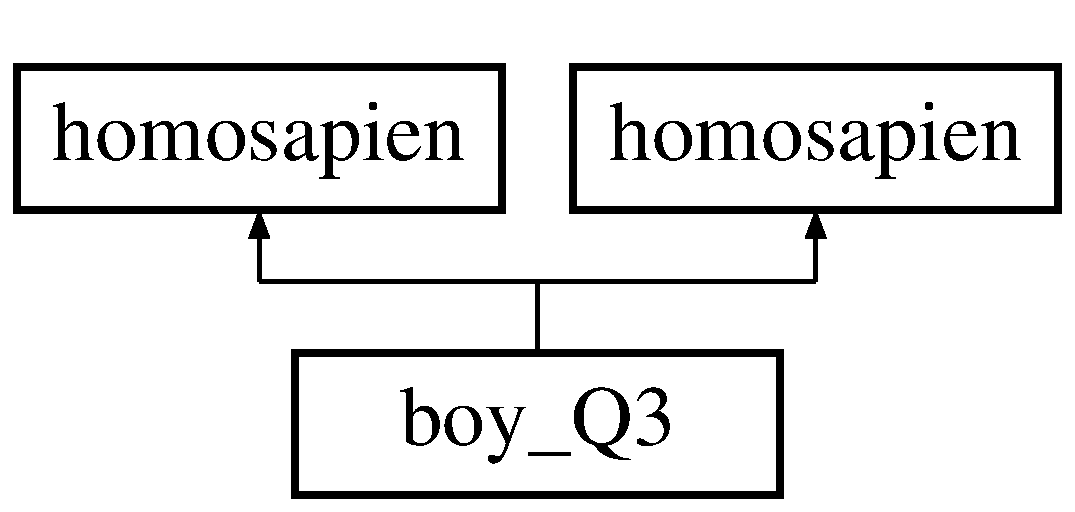
\includegraphics[height=2.000000cm]{classboy___q3}
\end{center}
\end{figure}
\subsection*{Public Member Functions}
\begin{DoxyCompactItemize}
\item 
\hyperlink{classboy___q3_a18bbddd5a186cc05ec12d7e9213924b4}{boy\+\_\+\+Q3} (std\+::string, int, int, int, bool, int, int)
\begin{DoxyCompactList}\small\item\em boy minimum attractiveness \end{DoxyCompactList}\item 
void \hyperlink{classboy___q3_a7f642a510e5cd0878a7851b2b08ecdaf}{set\+Min\+\_\+attract} (int)
\begin{DoxyCompactList}\small\item\em constructor \end{DoxyCompactList}\item 
int \hyperlink{classboy___q3_adf326922fe56a18158161d0d41ebfe6d}{get\+Min\+\_\+attract} (void)
\item 
\hyperlink{classboy___q3}{boy\+\_\+\+Q3}(std\+::string, int, int, int, bool, int, int) void \hyperlink{classboy___q3_aeed82f5c07060bc8292dd4f119b70e00}{set\+Min\+\_\+attract} (int)
\begin{DoxyCompactList}\small\item\em boy minimum attractiveness \end{DoxyCompactList}\item 
int \hyperlink{classboy___q3_adf326922fe56a18158161d0d41ebfe6d}{get\+Min\+\_\+attract} (void)
\end{DoxyCompactItemize}
\subsection*{Additional Inherited Members}


\subsection{Constructor \& Destructor Documentation}
\mbox{\Hypertarget{classboy___q3_a18bbddd5a186cc05ec12d7e9213924b4}\label{classboy___q3_a18bbddd5a186cc05ec12d7e9213924b4}} 
\index{boy\+\_\+\+Q3@{boy\+\_\+\+Q3}!boy\+\_\+\+Q3@{boy\+\_\+\+Q3}}
\index{boy\+\_\+\+Q3@{boy\+\_\+\+Q3}!boy\+\_\+\+Q3@{boy\+\_\+\+Q3}}
\subsubsection{\texorpdfstring{boy\+\_\+\+Q3()}{boy\_Q3()}}
{\footnotesize\ttfamily boy\+\_\+\+Q3\+::boy\+\_\+\+Q3 (\begin{DoxyParamCaption}\item[{std\+::string}]{name,  }\item[{int}]{attractiveness,  }\item[{int}]{intelligence,  }\item[{int}]{min\+\_\+attract,  }\item[{bool}]{is\+Commited,  }\item[{int}]{type,  }\item[{int}]{budget }\end{DoxyParamCaption})}



boy minimum attractiveness 

constructor that calls constructor of parent itself 

\subsection{Member Function Documentation}
\mbox{\Hypertarget{classboy___q3_adf326922fe56a18158161d0d41ebfe6d}\label{classboy___q3_adf326922fe56a18158161d0d41ebfe6d}} 
\index{boy\+\_\+\+Q3@{boy\+\_\+\+Q3}!get\+Min\+\_\+attract@{get\+Min\+\_\+attract}}
\index{get\+Min\+\_\+attract@{get\+Min\+\_\+attract}!boy\+\_\+\+Q3@{boy\+\_\+\+Q3}}
\subsubsection{\texorpdfstring{get\+Min\+\_\+attract()}{getMin\_attract()}\hspace{0.1cm}{\footnotesize\ttfamily [1/2]}}
{\footnotesize\ttfamily int boy\+\_\+\+Q3\+::get\+Min\+\_\+attract (\begin{DoxyParamCaption}\item[{void}]{ }\end{DoxyParamCaption})}

\mbox{\Hypertarget{classboy___q3_adf326922fe56a18158161d0d41ebfe6d}\label{classboy___q3_adf326922fe56a18158161d0d41ebfe6d}} 
\index{boy\+\_\+\+Q3@{boy\+\_\+\+Q3}!get\+Min\+\_\+attract@{get\+Min\+\_\+attract}}
\index{get\+Min\+\_\+attract@{get\+Min\+\_\+attract}!boy\+\_\+\+Q3@{boy\+\_\+\+Q3}}
\subsubsection{\texorpdfstring{get\+Min\+\_\+attract()}{getMin\_attract()}\hspace{0.1cm}{\footnotesize\ttfamily [2/2]}}
{\footnotesize\ttfamily int boy\+\_\+\+Q3\+::get\+Min\+\_\+attract (\begin{DoxyParamCaption}\item[{void}]{ }\end{DoxyParamCaption})}

\mbox{\Hypertarget{classboy___q3_aeed82f5c07060bc8292dd4f119b70e00}\label{classboy___q3_aeed82f5c07060bc8292dd4f119b70e00}} 
\index{boy\+\_\+\+Q3@{boy\+\_\+\+Q3}!set\+Min\+\_\+attract@{set\+Min\+\_\+attract}}
\index{set\+Min\+\_\+attract@{set\+Min\+\_\+attract}!boy\+\_\+\+Q3@{boy\+\_\+\+Q3}}
\subsubsection{\texorpdfstring{set\+Min\+\_\+attract()}{setMin\_attract()}\hspace{0.1cm}{\footnotesize\ttfamily [1/2]}}
{\footnotesize\ttfamily \hyperlink{classboy___q3}{boy\+\_\+\+Q3} (std\+::string,int,int,int,bool,int,int) void boy\+\_\+\+Q3\+::set\+Min\+\_\+attract (\begin{DoxyParamCaption}\item[{int}]{ }\end{DoxyParamCaption})}



boy minimum attractiveness 

constructor \mbox{\Hypertarget{classboy___q3_a7f642a510e5cd0878a7851b2b08ecdaf}\label{classboy___q3_a7f642a510e5cd0878a7851b2b08ecdaf}} 
\index{boy\+\_\+\+Q3@{boy\+\_\+\+Q3}!set\+Min\+\_\+attract@{set\+Min\+\_\+attract}}
\index{set\+Min\+\_\+attract@{set\+Min\+\_\+attract}!boy\+\_\+\+Q3@{boy\+\_\+\+Q3}}
\subsubsection{\texorpdfstring{set\+Min\+\_\+attract()}{setMin\_attract()}\hspace{0.1cm}{\footnotesize\ttfamily [2/2]}}
{\footnotesize\ttfamily void boy\+\_\+\+Q3\+::set\+Min\+\_\+attract (\begin{DoxyParamCaption}\item[{int}]{min\+\_\+attract }\end{DoxyParamCaption})}



constructor 



The documentation for this class was generated from the following files\+:\begin{DoxyCompactItemize}
\item 
\hyperlink{boy___q3_8h}{boy\+\_\+\+Q3.\+h}\item 
\hyperlink{boy___q3_8cpp}{boy\+\_\+\+Q3.\+cpp}\end{DoxyCompactItemize}

\hypertarget{classbreakup}{}\section{breakup Class Reference}
\label{classbreakup}\index{breakup@{breakup}}


{\ttfamily \#include $<$breakup.\+h$>$}

\subsection*{Friends}
\begin{DoxyCompactItemize}
\item 
void \hyperlink{classbreakup_a72fa040ab00ddfad8b81bda5bf4a7ff4}{break\+Up} (std\+::vector$<$ \hyperlink{classrel}{rel} $>$ \&r, std\+::vector$<$ \hyperlink{classboy}{boy} $>$ \&b, int kin, int t)
\end{DoxyCompactItemize}


\subsection{Friends And Related Function Documentation}
\mbox{\Hypertarget{classbreakup_a72fa040ab00ddfad8b81bda5bf4a7ff4}\label{classbreakup_a72fa040ab00ddfad8b81bda5bf4a7ff4}} 
\index{breakup@{breakup}!break\+Up@{break\+Up}}
\index{break\+Up@{break\+Up}!breakup@{breakup}}
\subsubsection{\texorpdfstring{break\+Up}{breakUp}}
{\footnotesize\ttfamily void break\+Up (\begin{DoxyParamCaption}\item[{std\+::vector$<$ \hyperlink{classrel}{rel} $>$ \&}]{r,  }\item[{std\+::vector$<$ \hyperlink{classboy}{boy} $>$ \&}]{b,  }\item[{int}]{kin,  }\item[{int}]{t }\end{DoxyParamCaption})\hspace{0.3cm}{\ttfamily [friend]}}



The documentation for this class was generated from the following file\+:\begin{DoxyCompactItemize}
\item 
\hyperlink{breakup_8h}{breakup.\+h}\end{DoxyCompactItemize}

\hypertarget{structcp}{}\section{cp Struct Reference}
\label{structcp}\index{cp@{cp}}
\subsection*{Public Attributes}
\begin{DoxyCompactItemize}
\item 
string \hyperlink{structcp_a5c0f14498ef91b80df382a4fa0ff07a6}{bname}
\item 
string \hyperlink{structcp_a778f4ec05a16b4c88a219f3e800d1aac}{gname}
\end{DoxyCompactItemize}


\subsection{Member Data Documentation}
\mbox{\Hypertarget{structcp_a5c0f14498ef91b80df382a4fa0ff07a6}\label{structcp_a5c0f14498ef91b80df382a4fa0ff07a6}} 
\index{cp@{cp}!bname@{bname}}
\index{bname@{bname}!cp@{cp}}
\subsubsection{\texorpdfstring{bname}{bname}}
{\footnotesize\ttfamily string cp\+::bname}

\mbox{\Hypertarget{structcp_a778f4ec05a16b4c88a219f3e800d1aac}\label{structcp_a778f4ec05a16b4c88a219f3e800d1aac}} 
\index{cp@{cp}!gname@{gname}}
\index{gname@{gname}!cp@{cp}}
\subsubsection{\texorpdfstring{gname}{gname}}
{\footnotesize\ttfamily string cp\+::gname}



The documentation for this struct was generated from the following file\+:\begin{DoxyCompactItemize}
\item 
\hyperlink{getgf_8cpp}{getgf.\+cpp}\end{DoxyCompactItemize}

\hypertarget{classgetgf}{}\section{getgf Class Reference}
\label{classgetgf}\index{getgf@{getgf}}


{\ttfamily \#include $<$getgf.\+h$>$}

\subsection*{Friends}
\begin{DoxyCompactItemize}
\item 
void \hyperlink{classgetgf_a1ca07cd41f0f09642e9982bd209133ce}{get\+Girl} (std\+::vector$<$ \hyperlink{classboy}{boy} $>$ \&b)
\end{DoxyCompactItemize}


\subsection{Friends And Related Function Documentation}
\mbox{\Hypertarget{classgetgf_a1ca07cd41f0f09642e9982bd209133ce}\label{classgetgf_a1ca07cd41f0f09642e9982bd209133ce}} 
\index{getgf@{getgf}!get\+Girl@{get\+Girl}}
\index{get\+Girl@{get\+Girl}!getgf@{getgf}}
\subsubsection{\texorpdfstring{get\+Girl}{getGirl}}
{\footnotesize\ttfamily void get\+Girl (\begin{DoxyParamCaption}\item[{std\+::vector$<$ \hyperlink{classboy}{boy} $>$ \&}]{b }\end{DoxyParamCaption})\hspace{0.3cm}{\ttfamily [friend]}}



The documentation for this class was generated from the following file\+:\begin{DoxyCompactItemize}
\item 
\hyperlink{getgf_8h}{getgf.\+h}\end{DoxyCompactItemize}

\hypertarget{classgift}{}\section{gift Class Reference}
\label{classgift}\index{gift@{gift}}
\subsection*{Public Member Functions}
\begin{DoxyCompactItemize}
\item 
\hyperlink{classgift_a782f5cf6316f6c76061b72cc12c6d95c}{gift} (int, double)
\begin{DoxyCompactList}\small\item\em var to check if gift is allocated \end{DoxyCompactList}\item 
\hyperlink{classgift_a1de4cec7237a45096900754354d1edb6}{gift} (int, double, int, int)
\begin{DoxyCompactList}\small\item\em constructor essential gift \end{DoxyCompactList}\item 
\hyperlink{classgift_ac62aba6ac2db2845c7b60a5496b6de75}{gift} (int, double, int, float)
\begin{DoxyCompactList}\small\item\em constructor luxury gift \end{DoxyCompactList}\item 
\mbox{\Hypertarget{classgift_a75432abfdbeec0b8880f4f3d265d41a6}\label{classgift_a75432abfdbeec0b8880f4f3d265d41a6}} 
int \hyperlink{classgift_a75432abfdbeec0b8880f4f3d265d41a6}{get\+Value} (void)
\begin{DoxyCompactList}\small\item\em constructor utility gift \end{DoxyCompactList}\item 
\mbox{\Hypertarget{classgift_afb3ea488ce0a02ae622c1acf5608bc94}\label{classgift_afb3ea488ce0a02ae622c1acf5608bc94}} 
double {\bfseries get\+Price} (void)
\item 
\mbox{\Hypertarget{classgift_a680a1bc8854391b628a36faa9568f790}\label{classgift_a680a1bc8854391b628a36faa9568f790}} 
int {\bfseries get\+Lux\+\_\+rat} (void)
\item 
\mbox{\Hypertarget{classgift_a677b7f1368eef76f344b3a623fdea915}\label{classgift_a677b7f1368eef76f344b3a623fdea915}} 
int {\bfseries get\+Difficulty} (void)
\item 
\mbox{\Hypertarget{classgift_a820ca25bbee4873ef9b0e82ca2f73ad3}\label{classgift_a820ca25bbee4873ef9b0e82ca2f73ad3}} 
int {\bfseries get\+Type} (void)
\item 
\mbox{\Hypertarget{classgift_a5e2d84e4d1fe8c00903a71195fc41487}\label{classgift_a5e2d84e4d1fe8c00903a71195fc41487}} 
int {\bfseries get\+Util\+\_\+val} (void)
\item 
\mbox{\Hypertarget{classgift_a2bb6e0ed9bb5c1f98d47660d39ebf3f8}\label{classgift_a2bb6e0ed9bb5c1f98d47660d39ebf3f8}} 
float {\bfseries get\+Util\+\_\+class} (void)
\item 
\mbox{\Hypertarget{classgift_a35e47e5084f539114e84b7ce477d93e2}\label{classgift_a35e47e5084f539114e84b7ce477d93e2}} 
int {\bfseries get\+Alc} (void)
\item 
\mbox{\Hypertarget{classgift_a312e5d347516d8ea351e1127de8a28ce}\label{classgift_a312e5d347516d8ea351e1127de8a28ce}} 
void {\bfseries set\+Alc} (void)
\end{DoxyCompactItemize}


\subsection{Constructor \& Destructor Documentation}
\mbox{\Hypertarget{classgift_a782f5cf6316f6c76061b72cc12c6d95c}\label{classgift_a782f5cf6316f6c76061b72cc12c6d95c}} 
\index{gift@{gift}!gift@{gift}}
\index{gift@{gift}!gift@{gift}}
\subsubsection{\texorpdfstring{gift()}{gift()}\hspace{0.1cm}{\footnotesize\ttfamily [1/3]}}
{\footnotesize\ttfamily gift\+::gift (\begin{DoxyParamCaption}\item[{int}]{value,  }\item[{double}]{price }\end{DoxyParamCaption})}



var to check if gift is allocated 

constructor essential gift \mbox{\Hypertarget{classgift_a1de4cec7237a45096900754354d1edb6}\label{classgift_a1de4cec7237a45096900754354d1edb6}} 
\index{gift@{gift}!gift@{gift}}
\index{gift@{gift}!gift@{gift}}
\subsubsection{\texorpdfstring{gift()}{gift()}\hspace{0.1cm}{\footnotesize\ttfamily [2/3]}}
{\footnotesize\ttfamily gift\+::gift (\begin{DoxyParamCaption}\item[{int}]{value,  }\item[{double}]{price,  }\item[{int}]{lux\+\_\+rat,  }\item[{int}]{difficulty }\end{DoxyParamCaption})}



constructor essential gift 

constructor luxury gift \mbox{\Hypertarget{classgift_ac62aba6ac2db2845c7b60a5496b6de75}\label{classgift_ac62aba6ac2db2845c7b60a5496b6de75}} 
\index{gift@{gift}!gift@{gift}}
\index{gift@{gift}!gift@{gift}}
\subsubsection{\texorpdfstring{gift()}{gift()}\hspace{0.1cm}{\footnotesize\ttfamily [3/3]}}
{\footnotesize\ttfamily gift\+::gift (\begin{DoxyParamCaption}\item[{int}]{value,  }\item[{double}]{price,  }\item[{int}]{util\+\_\+val,  }\item[{float}]{util\+\_\+class }\end{DoxyParamCaption})}



constructor luxury gift 

constructor utility gift 

The documentation for this class was generated from the following files\+:\begin{DoxyCompactItemize}
\item 
gift.\+h\item 
gift.\+cpp\end{DoxyCompactItemize}

\hypertarget{classgirl}{}\section{girl Class Reference}
\label{classgirl}\index{girl@{girl}}


{\ttfamily \#include $<$girl.\+h$>$}

\subsection*{Public Member Functions}
\begin{DoxyCompactItemize}
\item 
\hyperlink{classgirl_a583ce9589214531dc92c46e9d0eebc75}{girl} (std\+::string, int, int, bool, int, int, int)
\item 
void \hyperlink{classgirl_acbf8f5cee4f0cf24df3c96fc43666b43}{set\+Name} (std\+::string)
\begin{DoxyCompactList}\small\item\em constructor \end{DoxyCompactList}\item 
void \hyperlink{classgirl_a631115234a7e2ca7b497856e32c4ee7b}{set\+Attractiveness} (int)
\item 
void \hyperlink{classgirl_a3a4c341525032ef1a9a43572ab4ab370}{set\+Intelligence} (int)
\item 
void \hyperlink{classgirl_aa02816fb19d2f81683b5fe75729eacb1}{set\+Is\+\_\+commited} (bool)
\item 
void \hyperlink{classgirl_a761660d73115bf5940576daab5719aff}{set\+Boyname} (std\+::string)
\item 
void \hyperlink{classgirl_a85b694210361853ec1fee3f232491009}{set\+Type} (int)
\item 
void \hyperlink{classgirl_afdd10cabb120b9bbc44c8c243168baf3}{set\+Preference} (int)
\item 
void \hyperlink{classgirl_aabb69c46aef35ff020d90d3b28300f98}{set\+Budget} (int)
\item 
std\+::string \hyperlink{classgirl_ae0499077a33b4a517867f431bccfe93a}{get\+Name} (void)
\item 
int \hyperlink{classgirl_a25c8b2bc2d3df50ca61417f0e8c4eef5}{get\+Attractiveness} (void)
\item 
int \hyperlink{classgirl_a7cd49c129d9ede212cf24a0d93bfcc6a}{get\+Intelligence} (void)
\item 
int \hyperlink{classgirl_aa1565f1f255770e69de297bb631a4ed8}{get\+Is\+\_\+commited} (void)
\item 
int \hyperlink{classgirl_ac0eb402f33a9b066a89ae0eeda483ea4}{get\+Type} (void)
\item 
int \hyperlink{classgirl_a445487f05d077114171887781a12e151}{get\+Preference} (void)
\item 
int \hyperlink{classgirl_aff71d37b752b3501114356f862ae91a3}{get\+Budget} (void)
\end{DoxyCompactItemize}
\subsection*{Public Attributes}
\begin{DoxyCompactItemize}
\item 
int \hyperlink{classgirl_a0d038ec12424d8b11fa0442bfa6fe2d6}{maintenance\+\_\+budget}
\begin{DoxyCompactList}\small\item\em girl preference \textquotesingle{}1\textquotesingle{} = most rich \textquotesingle{}2\textquotesingle{} = most attractive \textquotesingle{}3\textquotesingle{} = most intelligent \end{DoxyCompactList}\end{DoxyCompactItemize}


\subsection{Constructor \& Destructor Documentation}
\mbox{\Hypertarget{classgirl_a583ce9589214531dc92c46e9d0eebc75}\label{classgirl_a583ce9589214531dc92c46e9d0eebc75}} 
\index{girl@{girl}!girl@{girl}}
\index{girl@{girl}!girl@{girl}}
\subsubsection{\texorpdfstring{girl()}{girl()}}
{\footnotesize\ttfamily girl\+::girl (\begin{DoxyParamCaption}\item[{std\+::string}]{name,  }\item[{int}]{attractiveness,  }\item[{int}]{intelligence,  }\item[{bool}]{is\+\_\+commited,  }\item[{int}]{type,  }\item[{int}]{pref,  }\item[{int}]{maintenance\+\_\+budget }\end{DoxyParamCaption})}

constructor 

\subsection{Member Function Documentation}
\mbox{\Hypertarget{classgirl_a25c8b2bc2d3df50ca61417f0e8c4eef5}\label{classgirl_a25c8b2bc2d3df50ca61417f0e8c4eef5}} 
\index{girl@{girl}!get\+Attractiveness@{get\+Attractiveness}}
\index{get\+Attractiveness@{get\+Attractiveness}!girl@{girl}}
\subsubsection{\texorpdfstring{get\+Attractiveness()}{getAttractiveness()}}
{\footnotesize\ttfamily int girl\+::get\+Attractiveness (\begin{DoxyParamCaption}\item[{void}]{ }\end{DoxyParamCaption})}

\mbox{\Hypertarget{classgirl_aff71d37b752b3501114356f862ae91a3}\label{classgirl_aff71d37b752b3501114356f862ae91a3}} 
\index{girl@{girl}!get\+Budget@{get\+Budget}}
\index{get\+Budget@{get\+Budget}!girl@{girl}}
\subsubsection{\texorpdfstring{get\+Budget()}{getBudget()}}
{\footnotesize\ttfamily int girl\+::get\+Budget (\begin{DoxyParamCaption}\item[{void}]{ }\end{DoxyParamCaption})}

\mbox{\Hypertarget{classgirl_a7cd49c129d9ede212cf24a0d93bfcc6a}\label{classgirl_a7cd49c129d9ede212cf24a0d93bfcc6a}} 
\index{girl@{girl}!get\+Intelligence@{get\+Intelligence}}
\index{get\+Intelligence@{get\+Intelligence}!girl@{girl}}
\subsubsection{\texorpdfstring{get\+Intelligence()}{getIntelligence()}}
{\footnotesize\ttfamily int girl\+::get\+Intelligence (\begin{DoxyParamCaption}\item[{void}]{ }\end{DoxyParamCaption})}

\mbox{\Hypertarget{classgirl_aa1565f1f255770e69de297bb631a4ed8}\label{classgirl_aa1565f1f255770e69de297bb631a4ed8}} 
\index{girl@{girl}!get\+Is\+\_\+commited@{get\+Is\+\_\+commited}}
\index{get\+Is\+\_\+commited@{get\+Is\+\_\+commited}!girl@{girl}}
\subsubsection{\texorpdfstring{get\+Is\+\_\+commited()}{getIs\_commited()}}
{\footnotesize\ttfamily int girl\+::get\+Is\+\_\+commited (\begin{DoxyParamCaption}\item[{void}]{ }\end{DoxyParamCaption})}

\mbox{\Hypertarget{classgirl_ae0499077a33b4a517867f431bccfe93a}\label{classgirl_ae0499077a33b4a517867f431bccfe93a}} 
\index{girl@{girl}!get\+Name@{get\+Name}}
\index{get\+Name@{get\+Name}!girl@{girl}}
\subsubsection{\texorpdfstring{get\+Name()}{getName()}}
{\footnotesize\ttfamily std\+::string girl\+::get\+Name (\begin{DoxyParamCaption}\item[{void}]{ }\end{DoxyParamCaption})}

\mbox{\Hypertarget{classgirl_a445487f05d077114171887781a12e151}\label{classgirl_a445487f05d077114171887781a12e151}} 
\index{girl@{girl}!get\+Preference@{get\+Preference}}
\index{get\+Preference@{get\+Preference}!girl@{girl}}
\subsubsection{\texorpdfstring{get\+Preference()}{getPreference()}}
{\footnotesize\ttfamily int girl\+::get\+Preference (\begin{DoxyParamCaption}\item[{void}]{ }\end{DoxyParamCaption})}

\mbox{\Hypertarget{classgirl_ac0eb402f33a9b066a89ae0eeda483ea4}\label{classgirl_ac0eb402f33a9b066a89ae0eeda483ea4}} 
\index{girl@{girl}!get\+Type@{get\+Type}}
\index{get\+Type@{get\+Type}!girl@{girl}}
\subsubsection{\texorpdfstring{get\+Type()}{getType()}}
{\footnotesize\ttfamily int girl\+::get\+Type (\begin{DoxyParamCaption}\item[{void}]{ }\end{DoxyParamCaption})}

\mbox{\Hypertarget{classgirl_a631115234a7e2ca7b497856e32c4ee7b}\label{classgirl_a631115234a7e2ca7b497856e32c4ee7b}} 
\index{girl@{girl}!set\+Attractiveness@{set\+Attractiveness}}
\index{set\+Attractiveness@{set\+Attractiveness}!girl@{girl}}
\subsubsection{\texorpdfstring{set\+Attractiveness()}{setAttractiveness()}}
{\footnotesize\ttfamily void girl\+::set\+Attractiveness (\begin{DoxyParamCaption}\item[{int}]{attractiveness }\end{DoxyParamCaption})}

\mbox{\Hypertarget{classgirl_a761660d73115bf5940576daab5719aff}\label{classgirl_a761660d73115bf5940576daab5719aff}} 
\index{girl@{girl}!set\+Boyname@{set\+Boyname}}
\index{set\+Boyname@{set\+Boyname}!girl@{girl}}
\subsubsection{\texorpdfstring{set\+Boyname()}{setBoyname()}}
{\footnotesize\ttfamily void girl\+::set\+Boyname (\begin{DoxyParamCaption}\item[{std\+::string}]{ }\end{DoxyParamCaption})}

\mbox{\Hypertarget{classgirl_aabb69c46aef35ff020d90d3b28300f98}\label{classgirl_aabb69c46aef35ff020d90d3b28300f98}} 
\index{girl@{girl}!set\+Budget@{set\+Budget}}
\index{set\+Budget@{set\+Budget}!girl@{girl}}
\subsubsection{\texorpdfstring{set\+Budget()}{setBudget()}}
{\footnotesize\ttfamily void girl\+::set\+Budget (\begin{DoxyParamCaption}\item[{int}]{maintenance\+\_\+budget }\end{DoxyParamCaption})}

\mbox{\Hypertarget{classgirl_a3a4c341525032ef1a9a43572ab4ab370}\label{classgirl_a3a4c341525032ef1a9a43572ab4ab370}} 
\index{girl@{girl}!set\+Intelligence@{set\+Intelligence}}
\index{set\+Intelligence@{set\+Intelligence}!girl@{girl}}
\subsubsection{\texorpdfstring{set\+Intelligence()}{setIntelligence()}}
{\footnotesize\ttfamily void girl\+::set\+Intelligence (\begin{DoxyParamCaption}\item[{int}]{intelligence }\end{DoxyParamCaption})}

\mbox{\Hypertarget{classgirl_aa02816fb19d2f81683b5fe75729eacb1}\label{classgirl_aa02816fb19d2f81683b5fe75729eacb1}} 
\index{girl@{girl}!set\+Is\+\_\+commited@{set\+Is\+\_\+commited}}
\index{set\+Is\+\_\+commited@{set\+Is\+\_\+commited}!girl@{girl}}
\subsubsection{\texorpdfstring{set\+Is\+\_\+commited()}{setIs\_commited()}}
{\footnotesize\ttfamily void girl\+::set\+Is\+\_\+commited (\begin{DoxyParamCaption}\item[{bool}]{is\+\_\+commited }\end{DoxyParamCaption})}

\mbox{\Hypertarget{classgirl_acbf8f5cee4f0cf24df3c96fc43666b43}\label{classgirl_acbf8f5cee4f0cf24df3c96fc43666b43}} 
\index{girl@{girl}!set\+Name@{set\+Name}}
\index{set\+Name@{set\+Name}!girl@{girl}}
\subsubsection{\texorpdfstring{set\+Name()}{setName()}}
{\footnotesize\ttfamily void girl\+::set\+Name (\begin{DoxyParamCaption}\item[{std\+::string}]{name }\end{DoxyParamCaption})}



constructor 

\mbox{\Hypertarget{classgirl_afdd10cabb120b9bbc44c8c243168baf3}\label{classgirl_afdd10cabb120b9bbc44c8c243168baf3}} 
\index{girl@{girl}!set\+Preference@{set\+Preference}}
\index{set\+Preference@{set\+Preference}!girl@{girl}}
\subsubsection{\texorpdfstring{set\+Preference()}{setPreference()}}
{\footnotesize\ttfamily void girl\+::set\+Preference (\begin{DoxyParamCaption}\item[{int}]{pref }\end{DoxyParamCaption})}

\mbox{\Hypertarget{classgirl_a85b694210361853ec1fee3f232491009}\label{classgirl_a85b694210361853ec1fee3f232491009}} 
\index{girl@{girl}!set\+Type@{set\+Type}}
\index{set\+Type@{set\+Type}!girl@{girl}}
\subsubsection{\texorpdfstring{set\+Type()}{setType()}}
{\footnotesize\ttfamily void girl\+::set\+Type (\begin{DoxyParamCaption}\item[{int}]{type }\end{DoxyParamCaption})}



\subsection{Member Data Documentation}
\mbox{\Hypertarget{classgirl_a0d038ec12424d8b11fa0442bfa6fe2d6}\label{classgirl_a0d038ec12424d8b11fa0442bfa6fe2d6}} 
\index{girl@{girl}!maintenance\+\_\+budget@{maintenance\+\_\+budget}}
\index{maintenance\+\_\+budget@{maintenance\+\_\+budget}!girl@{girl}}
\subsubsection{\texorpdfstring{maintenance\+\_\+budget}{maintenance\_budget}}
{\footnotesize\ttfamily int girl\+::maintenance\+\_\+budget}



girl preference \textquotesingle{}1\textquotesingle{} = most rich \textquotesingle{}2\textquotesingle{} = most attractive \textquotesingle{}3\textquotesingle{} = most intelligent 



The documentation for this class was generated from the following files\+:\begin{DoxyCompactItemize}
\item 
\hyperlink{girl_8h}{girl.\+h}\item 
\hyperlink{girl_8cpp}{girl.\+cpp}\end{DoxyCompactItemize}

\hypertarget{classgirl___q3}{}\section{girl\+\_\+\+Q3 Class Reference}
\label{classgirl___q3}\index{girl\+\_\+\+Q3@{girl\+\_\+\+Q3}}


{\ttfamily \#include $<$girl\+\_\+\+Q3.\+h$>$}

Inheritance diagram for girl\+\_\+\+Q3\+:\begin{figure}[H]
\begin{center}
\leavevmode
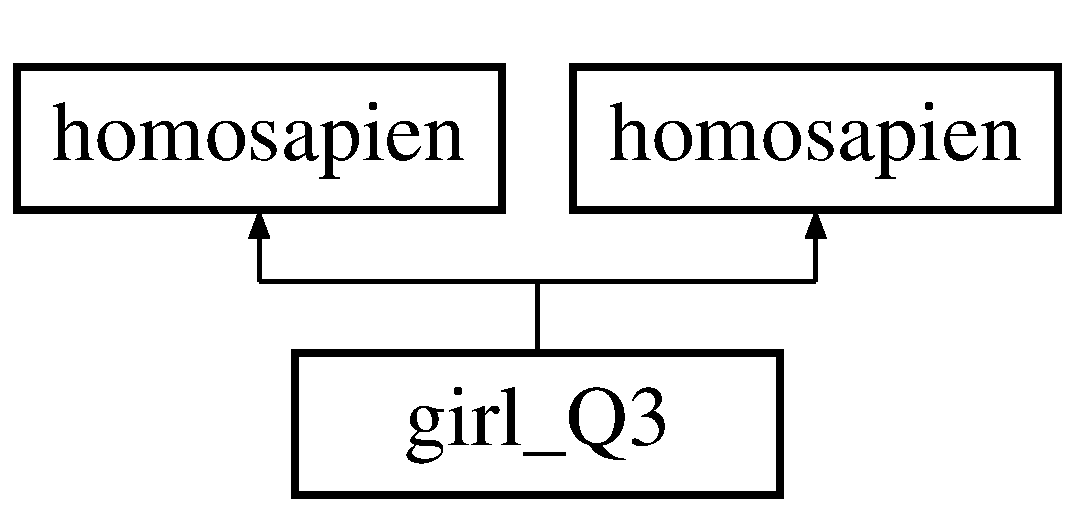
\includegraphics[height=2.000000cm]{classgirl___q3}
\end{center}
\end{figure}
\subsection*{Public Member Functions}
\begin{DoxyCompactItemize}
\item 
\hyperlink{classgirl___q3_a2c595ffa07045ad1d7d22ffcc36723a7}{girl\+\_\+\+Q3} (std\+::string, int, int, int, bool, int, int)
\begin{DoxyCompactList}\small\item\em girl preference \textquotesingle{}1\textquotesingle{} = most rich \textquotesingle{}2\textquotesingle{} = most attractive \textquotesingle{}3\textquotesingle{} = most intelligent \end{DoxyCompactList}\item 
void \hyperlink{classgirl___q3_a63eb2d16b6ea6c9c136b376bdfc1c85b}{set\+Preference} (int)
\begin{DoxyCompactList}\small\item\em constructor \end{DoxyCompactList}\item 
int \hyperlink{classgirl___q3_a95dbbddc79b5155a877e12e6352e08af}{get\+Preference} (void)
\item 
\hyperlink{classgirl___q3}{girl\+\_\+\+Q3}(std\+::string, int, int, int, bool, int, int) void \hyperlink{classgirl___q3_aeda05a4272fa1b371c7bbb2285b64e63}{set\+Preference} (int)
\begin{DoxyCompactList}\small\item\em girl preference \textquotesingle{}1\textquotesingle{} = most rich \textquotesingle{}2\textquotesingle{} = most attractive \textquotesingle{}3\textquotesingle{} = most intelligent \end{DoxyCompactList}\item 
int \hyperlink{classgirl___q3_a95dbbddc79b5155a877e12e6352e08af}{get\+Preference} (void)
\end{DoxyCompactItemize}
\subsection*{Additional Inherited Members}


\subsection{Constructor \& Destructor Documentation}
\mbox{\Hypertarget{classgirl___q3_a2c595ffa07045ad1d7d22ffcc36723a7}\label{classgirl___q3_a2c595ffa07045ad1d7d22ffcc36723a7}} 
\index{girl\+\_\+\+Q3@{girl\+\_\+\+Q3}!girl\+\_\+\+Q3@{girl\+\_\+\+Q3}}
\index{girl\+\_\+\+Q3@{girl\+\_\+\+Q3}!girl\+\_\+\+Q3@{girl\+\_\+\+Q3}}
\subsubsection{\texorpdfstring{girl\+\_\+\+Q3()}{girl\_Q3()}}
{\footnotesize\ttfamily girl\+\_\+\+Q3\+::girl\+\_\+\+Q3 (\begin{DoxyParamCaption}\item[{std\+::string}]{name,  }\item[{int}]{attractiveness,  }\item[{int}]{intelligence,  }\item[{int}]{pref,  }\item[{bool}]{is\+Commited,  }\item[{int}]{type,  }\item[{int}]{budget }\end{DoxyParamCaption})}



girl preference \textquotesingle{}1\textquotesingle{} = most rich \textquotesingle{}2\textquotesingle{} = most attractive \textquotesingle{}3\textquotesingle{} = most intelligent 

constructor that calls parent constructor itseld 

\subsection{Member Function Documentation}
\mbox{\Hypertarget{classgirl___q3_a95dbbddc79b5155a877e12e6352e08af}\label{classgirl___q3_a95dbbddc79b5155a877e12e6352e08af}} 
\index{girl\+\_\+\+Q3@{girl\+\_\+\+Q3}!get\+Preference@{get\+Preference}}
\index{get\+Preference@{get\+Preference}!girl\+\_\+\+Q3@{girl\+\_\+\+Q3}}
\subsubsection{\texorpdfstring{get\+Preference()}{getPreference()}\hspace{0.1cm}{\footnotesize\ttfamily [1/2]}}
{\footnotesize\ttfamily int girl\+\_\+\+Q3\+::get\+Preference (\begin{DoxyParamCaption}\item[{void}]{ }\end{DoxyParamCaption})}

\mbox{\Hypertarget{classgirl___q3_a95dbbddc79b5155a877e12e6352e08af}\label{classgirl___q3_a95dbbddc79b5155a877e12e6352e08af}} 
\index{girl\+\_\+\+Q3@{girl\+\_\+\+Q3}!get\+Preference@{get\+Preference}}
\index{get\+Preference@{get\+Preference}!girl\+\_\+\+Q3@{girl\+\_\+\+Q3}}
\subsubsection{\texorpdfstring{get\+Preference()}{getPreference()}\hspace{0.1cm}{\footnotesize\ttfamily [2/2]}}
{\footnotesize\ttfamily int girl\+\_\+\+Q3\+::get\+Preference (\begin{DoxyParamCaption}\item[{void}]{ }\end{DoxyParamCaption})}

\mbox{\Hypertarget{classgirl___q3_aeda05a4272fa1b371c7bbb2285b64e63}\label{classgirl___q3_aeda05a4272fa1b371c7bbb2285b64e63}} 
\index{girl\+\_\+\+Q3@{girl\+\_\+\+Q3}!set\+Preference@{set\+Preference}}
\index{set\+Preference@{set\+Preference}!girl\+\_\+\+Q3@{girl\+\_\+\+Q3}}
\subsubsection{\texorpdfstring{set\+Preference()}{setPreference()}\hspace{0.1cm}{\footnotesize\ttfamily [1/2]}}
{\footnotesize\ttfamily \hyperlink{classgirl___q3}{girl\+\_\+\+Q3} (std\+::string,int,int,int,bool,int,int) void girl\+\_\+\+Q3\+::set\+Preference (\begin{DoxyParamCaption}\item[{int}]{ }\end{DoxyParamCaption})}



girl preference \textquotesingle{}1\textquotesingle{} = most rich \textquotesingle{}2\textquotesingle{} = most attractive \textquotesingle{}3\textquotesingle{} = most intelligent 

constructor \mbox{\Hypertarget{classgirl___q3_a63eb2d16b6ea6c9c136b376bdfc1c85b}\label{classgirl___q3_a63eb2d16b6ea6c9c136b376bdfc1c85b}} 
\index{girl\+\_\+\+Q3@{girl\+\_\+\+Q3}!set\+Preference@{set\+Preference}}
\index{set\+Preference@{set\+Preference}!girl\+\_\+\+Q3@{girl\+\_\+\+Q3}}
\subsubsection{\texorpdfstring{set\+Preference()}{setPreference()}\hspace{0.1cm}{\footnotesize\ttfamily [2/2]}}
{\footnotesize\ttfamily void girl\+\_\+\+Q3\+::set\+Preference (\begin{DoxyParamCaption}\item[{int}]{pref }\end{DoxyParamCaption})}



constructor 



The documentation for this class was generated from the following files\+:\begin{DoxyCompactItemize}
\item 
\hyperlink{girl___q3_8h}{girl\+\_\+\+Q3.\+h}\item 
\hyperlink{girl___q3_8cpp}{girl\+\_\+\+Q3.\+cpp}\end{DoxyCompactItemize}

\hypertarget{classgive__gift}{}\section{give\+\_\+gift Class Reference}
\label{classgive__gift}\index{give\+\_\+gift@{give\+\_\+gift}}


{\ttfamily \#include $<$give\+\_\+gift.\+h$>$}

\subsection*{Friends}
\begin{DoxyCompactItemize}
\item 
void \hyperlink{classgive__gift_a4d58aac625b116fce2965ee8ed463409}{give\+Gift} (std\+::vector$<$ \hyperlink{classgift}{gift} $>$ \&g, std\+::vector$<$ \hyperlink{classrel}{rel} $>$ \&r)
\begin{DoxyCompactList}\small\item\em friend keyword to make function usable by other classes \end{DoxyCompactList}\end{DoxyCompactItemize}


\subsection{Friends And Related Function Documentation}
\mbox{\Hypertarget{classgive__gift_a4d58aac625b116fce2965ee8ed463409}\label{classgive__gift_a4d58aac625b116fce2965ee8ed463409}} 
\index{give\+\_\+gift@{give\+\_\+gift}!give\+Gift@{give\+Gift}}
\index{give\+Gift@{give\+Gift}!give\+\_\+gift@{give\+\_\+gift}}
\subsubsection{\texorpdfstring{give\+Gift}{giveGift}}
{\footnotesize\ttfamily void give\+Gift (\begin{DoxyParamCaption}\item[{std\+::vector$<$ \hyperlink{classgift}{gift} $>$ \&}]{g,  }\item[{std\+::vector$<$ \hyperlink{classrel}{rel} $>$ \&}]{r }\end{DoxyParamCaption})\hspace{0.3cm}{\ttfamily [friend]}}



friend keyword to make function usable by other classes 

list of essential gifts

no of luxury gifts

no of essential gifts

no of utility gifts

list of utility gifts

list of luxury gifts

list of couples formed

x to flush of not important commas

calculate total price

calculate sum of values

calculate remaining budget

set gift to be allocated so that gift can no longer can be used

calculate happiness for girl type 1

calculate happiness for girl type 2

calculate happiness for girl type 3

calculate happiness for boy type 1

calculate happiness for boy type 2

calculate happiness for boy type 3

calculate couple happiness

calculate couple compatibility 

The documentation for this class was generated from the following file\+:\begin{DoxyCompactItemize}
\item 
\hyperlink{give__gift_8h}{give\+\_\+gift.\+h}\end{DoxyCompactItemize}

\hypertarget{classgive__gift___q5}{}\section{give\+\_\+gift\+\_\+\+Q5 Class Reference}
\label{classgive__gift___q5}\index{give\+\_\+gift\+\_\+\+Q5@{give\+\_\+gift\+\_\+\+Q5}}


{\ttfamily \#include $<$give\+\_\+gift\+\_\+\+Q5.\+h$>$}

\subsection*{Friends}
\begin{DoxyCompactItemize}
\item 
void \hyperlink{classgive__gift___q5_abad76b5070a0fdf9d34a475880a6a778}{give\+GiftQ} (std\+::vector$<$ \hyperlink{classgift}{gift} $>$ \&g, std\+::vector$<$ \hyperlink{classrel}{rel} $>$ \&r)
\end{DoxyCompactItemize}


\subsection{Friends And Related Function Documentation}
\mbox{\Hypertarget{classgive__gift___q5_abad76b5070a0fdf9d34a475880a6a778}\label{classgive__gift___q5_abad76b5070a0fdf9d34a475880a6a778}} 
\index{give\+\_\+gift\+\_\+\+Q5@{give\+\_\+gift\+\_\+\+Q5}!give\+GiftQ@{give\+GiftQ}}
\index{give\+GiftQ@{give\+GiftQ}!give\+\_\+gift\+\_\+\+Q5@{give\+\_\+gift\+\_\+\+Q5}}
\subsubsection{\texorpdfstring{give\+GiftQ}{giveGiftQ}}
{\footnotesize\ttfamily void give\+GiftQ (\begin{DoxyParamCaption}\item[{std\+::vector$<$ \hyperlink{classgift}{gift} $>$ \&}]{g,  }\item[{std\+::vector$<$ \hyperlink{classrel}{rel} $>$ \&}]{r }\end{DoxyParamCaption})\hspace{0.3cm}{\ttfamily [friend]}}

list of essential gifts

no of luxury gifts

no of essential gifts

no of utility gifts

list of utility gifts

list of luxury gifts

list of couples formed

x to flush of not important commas

calculate total price

calculate sum of values

calculate remaining budget

set gift to be allocated so that gift can no longer can be used

calculate happiness for girl type 1

calculate happiness for girl type 2

calculate happiness for girl type 3

calculate happiness for boy type 1

calculate happiness for boy type 2

calculate happiness for boy type 3

calculate couple happiness

calculate couple compatibility 

The documentation for this class was generated from the following file\+:\begin{DoxyCompactItemize}
\item 
\hyperlink{give__gift___q5_8h}{give\+\_\+gift\+\_\+\+Q5.\+h}\end{DoxyCompactItemize}

\hypertarget{classgive__new}{}\section{give\+\_\+new Class Reference}
\label{classgive__new}\index{give\+\_\+new@{give\+\_\+new}}


{\ttfamily \#include $<$give\+\_\+new.\+h$>$}

\subsection*{Friends}
\begin{DoxyCompactItemize}
\item 
void \hyperlink{classgive__new_a218ad00cb368ca7fdbe9d2201e9920bc}{give\+Al} (std\+::vector$<$ \hyperlink{classgift}{gift} $>$ \&ug, std\+::vector$<$ \hyperlink{classgift}{gift} $>$ \&eg, std\+::vector$<$ \hyperlink{classgift}{gift} $>$ \&lg, std\+::vector$<$ \hyperlink{classrel}{rel} $>$ \&r)
\end{DoxyCompactItemize}


\subsection{Friends And Related Function Documentation}
\mbox{\Hypertarget{classgive__new_a218ad00cb368ca7fdbe9d2201e9920bc}\label{classgive__new_a218ad00cb368ca7fdbe9d2201e9920bc}} 
\index{give\+\_\+new@{give\+\_\+new}!give\+Al@{give\+Al}}
\index{give\+Al@{give\+Al}!give\+\_\+new@{give\+\_\+new}}
\subsubsection{\texorpdfstring{give\+Al}{giveAl}}
{\footnotesize\ttfamily void give\+Al (\begin{DoxyParamCaption}\item[{std\+::vector$<$ \hyperlink{classgift}{gift} $>$ \&}]{ug,  }\item[{std\+::vector$<$ \hyperlink{classgift}{gift} $>$ \&}]{eg,  }\item[{std\+::vector$<$ \hyperlink{classgift}{gift} $>$ \&}]{lg,  }\item[{std\+::vector$<$ \hyperlink{classrel}{rel} $>$ \&}]{r }\end{DoxyParamCaption})\hspace{0.3cm}{\ttfamily [friend]}}

list of essential gifts

no of luxury gifts

no of essential gifts

no of utility gifts

list of utility gifts

list of luxury gifts

list of couples formed

x to flush of not important commas

calculate total price

calculate sum of values

calculate remaining budget

set gift to be allocated so that gift can no longer can be used

set gift to be allocated so that gift can no longer can be use

set gift to be allocated so that gift can no longer can be use

calculate happiness for girl type 1

calculate happiness for girl type 2

calculate happiness for girl type 3

calculate happiness for boy type 1

calculate happiness for boy type 2

calculate happiness for boy type 3

calculate couple happiness

calculate couple compatibility 

The documentation for this class was generated from the following file\+:\begin{DoxyCompactItemize}
\item 
\hyperlink{give__new_8h}{give\+\_\+new.\+h}\end{DoxyCompactItemize}

\hypertarget{classhomosapien}{}\section{homosapien Class Reference}
\label{classhomosapien}\index{homosapien@{homosapien}}


parent class of boy and girl  




{\ttfamily \#include $<$homosapien.\+h$>$}

Inheritance diagram for homosapien\+:\begin{figure}[H]
\begin{center}
\leavevmode
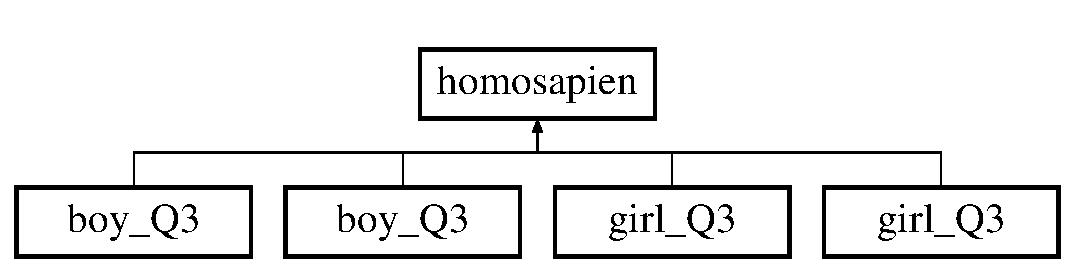
\includegraphics[height=2.000000cm]{classhomosapien}
\end{center}
\end{figure}
\subsection*{Public Member Functions}
\begin{DoxyCompactItemize}
\item 
\hyperlink{classhomosapien_a102098b80f8af39b27dafdff15d6aeee}{homosapien} (std\+::string, int, int, bool, int, int)
\begin{DoxyCompactList}\small\item\em boy budget \end{DoxyCompactList}\item 
void \hyperlink{classhomosapien_a0b0de2b72513ee20ba408ea29865e5f4}{set\+Name} (std\+::string)
\begin{DoxyCompactList}\small\item\em constructor \end{DoxyCompactList}\item 
void \hyperlink{classhomosapien_a264fd071fc5a6efda03730c34bfbc49c}{set\+Attractiveness} (int)
\item 
void \hyperlink{classhomosapien_adcfb3c7207fd77965679df8b85e5a507}{set\+Intelligence} (int)
\item 
void \hyperlink{classhomosapien_afee55d18c833bdfeac7392843e8580cc}{set\+Is\+\_\+commited} (bool)
\item 
void \hyperlink{classhomosapien_aa868001c96c4c26e5cbe85d7d75c738e}{set\+Type} (int)
\item 
void \hyperlink{classhomosapien_a3ad8cc4965cf29863337d0d56ca87d2d}{set\+Budget} (int)
\item 
std\+::string \hyperlink{classhomosapien_a1e93a89a2490a563289e7ad7a295ff45}{get\+Name} (void)
\item 
int \hyperlink{classhomosapien_a36bfd2262341cc01977ee077a7e5f619}{get\+Attractiveness} (void)
\item 
int \hyperlink{classhomosapien_ab9aa094786987a968b9a156a6d038931}{get\+Intelligence} (void)
\item 
int \hyperlink{classhomosapien_a3264f22c6b40fd138286980a7bafd11e}{get\+Is\+\_\+commited} (void)
\item 
int \hyperlink{classhomosapien_a2157c9d5eeb763c5fde1f42f4a6bb48b}{get\+Type} (void)
\item 
int \hyperlink{classhomosapien_a372c40e87592045235e89956ddda2488}{get\+Budget} (void)
\item 
\hyperlink{classhomosapien_a102098b80f8af39b27dafdff15d6aeee}{homosapien} (std\+::string, int, int, bool, int, int)
\begin{DoxyCompactList}\small\item\em human budget \end{DoxyCompactList}\item 
void \hyperlink{classhomosapien_a0b0de2b72513ee20ba408ea29865e5f4}{set\+Name} (std\+::string)
\begin{DoxyCompactList}\small\item\em constructor \end{DoxyCompactList}\item 
void \hyperlink{classhomosapien_a264fd071fc5a6efda03730c34bfbc49c}{set\+Attractiveness} (int)
\item 
void \hyperlink{classhomosapien_adcfb3c7207fd77965679df8b85e5a507}{set\+Intelligence} (int)
\item 
void \hyperlink{classhomosapien_afee55d18c833bdfeac7392843e8580cc}{set\+Is\+\_\+commited} (bool)
\item 
void \hyperlink{classhomosapien_aa868001c96c4c26e5cbe85d7d75c738e}{set\+Type} (int)
\item 
void \hyperlink{classhomosapien_a3ad8cc4965cf29863337d0d56ca87d2d}{set\+Budget} (int)
\item 
std\+::string \hyperlink{classhomosapien_a1e93a89a2490a563289e7ad7a295ff45}{get\+Name} (void)
\item 
int \hyperlink{classhomosapien_a36bfd2262341cc01977ee077a7e5f619}{get\+Attractiveness} (void)
\item 
int \hyperlink{classhomosapien_ab9aa094786987a968b9a156a6d038931}{get\+Intelligence} (void)
\item 
int \hyperlink{classhomosapien_a3264f22c6b40fd138286980a7bafd11e}{get\+Is\+\_\+commited} (void)
\item 
int \hyperlink{classhomosapien_a2157c9d5eeb763c5fde1f42f4a6bb48b}{get\+Type} (void)
\item 
int \hyperlink{classhomosapien_a372c40e87592045235e89956ddda2488}{get\+Budget} (void)
\end{DoxyCompactItemize}
\subsection*{Public Attributes}
\begin{DoxyCompactItemize}
\item 
int \hyperlink{classhomosapien_a8e16a7132ce68bb9026113200f7599ad}{budget}
\end{DoxyCompactItemize}


\subsection{Detailed Description}
parent class of boy and girl 

\subsection{Constructor \& Destructor Documentation}
\mbox{\Hypertarget{classhomosapien_a102098b80f8af39b27dafdff15d6aeee}\label{classhomosapien_a102098b80f8af39b27dafdff15d6aeee}} 
\index{homosapien@{homosapien}!homosapien@{homosapien}}
\index{homosapien@{homosapien}!homosapien@{homosapien}}
\subsubsection{\texorpdfstring{homosapien()}{homosapien()}\hspace{0.1cm}{\footnotesize\ttfamily [1/2]}}
{\footnotesize\ttfamily homosapien\+::homosapien (\begin{DoxyParamCaption}\item[{std\+::string}]{name,  }\item[{int}]{attractiveness,  }\item[{int}]{intelligence,  }\item[{bool}]{is\+\_\+commited,  }\item[{int}]{type,  }\item[{int}]{budget }\end{DoxyParamCaption})}



boy budget 

parent class of boy and girl constructor \mbox{\Hypertarget{classhomosapien_a102098b80f8af39b27dafdff15d6aeee}\label{classhomosapien_a102098b80f8af39b27dafdff15d6aeee}} 
\index{homosapien@{homosapien}!homosapien@{homosapien}}
\index{homosapien@{homosapien}!homosapien@{homosapien}}
\subsubsection{\texorpdfstring{homosapien()}{homosapien()}\hspace{0.1cm}{\footnotesize\ttfamily [2/2]}}
{\footnotesize\ttfamily homosapien\+::homosapien (\begin{DoxyParamCaption}\item[{std\+::string}]{,  }\item[{int}]{,  }\item[{int}]{,  }\item[{bool}]{,  }\item[{int}]{,  }\item[{int}]{ }\end{DoxyParamCaption})}



human budget 



\subsection{Member Function Documentation}
\mbox{\Hypertarget{classhomosapien_a36bfd2262341cc01977ee077a7e5f619}\label{classhomosapien_a36bfd2262341cc01977ee077a7e5f619}} 
\index{homosapien@{homosapien}!get\+Attractiveness@{get\+Attractiveness}}
\index{get\+Attractiveness@{get\+Attractiveness}!homosapien@{homosapien}}
\subsubsection{\texorpdfstring{get\+Attractiveness()}{getAttractiveness()}\hspace{0.1cm}{\footnotesize\ttfamily [1/2]}}
{\footnotesize\ttfamily int homosapien\+::get\+Attractiveness (\begin{DoxyParamCaption}\item[{void}]{ }\end{DoxyParamCaption})}

\mbox{\Hypertarget{classhomosapien_a36bfd2262341cc01977ee077a7e5f619}\label{classhomosapien_a36bfd2262341cc01977ee077a7e5f619}} 
\index{homosapien@{homosapien}!get\+Attractiveness@{get\+Attractiveness}}
\index{get\+Attractiveness@{get\+Attractiveness}!homosapien@{homosapien}}
\subsubsection{\texorpdfstring{get\+Attractiveness()}{getAttractiveness()}\hspace{0.1cm}{\footnotesize\ttfamily [2/2]}}
{\footnotesize\ttfamily int homosapien\+::get\+Attractiveness (\begin{DoxyParamCaption}\item[{void}]{ }\end{DoxyParamCaption})}

\mbox{\Hypertarget{classhomosapien_a372c40e87592045235e89956ddda2488}\label{classhomosapien_a372c40e87592045235e89956ddda2488}} 
\index{homosapien@{homosapien}!get\+Budget@{get\+Budget}}
\index{get\+Budget@{get\+Budget}!homosapien@{homosapien}}
\subsubsection{\texorpdfstring{get\+Budget()}{getBudget()}\hspace{0.1cm}{\footnotesize\ttfamily [1/2]}}
{\footnotesize\ttfamily int homosapien\+::get\+Budget (\begin{DoxyParamCaption}\item[{void}]{ }\end{DoxyParamCaption})}

\mbox{\Hypertarget{classhomosapien_a372c40e87592045235e89956ddda2488}\label{classhomosapien_a372c40e87592045235e89956ddda2488}} 
\index{homosapien@{homosapien}!get\+Budget@{get\+Budget}}
\index{get\+Budget@{get\+Budget}!homosapien@{homosapien}}
\subsubsection{\texorpdfstring{get\+Budget()}{getBudget()}\hspace{0.1cm}{\footnotesize\ttfamily [2/2]}}
{\footnotesize\ttfamily int homosapien\+::get\+Budget (\begin{DoxyParamCaption}\item[{void}]{ }\end{DoxyParamCaption})}

\mbox{\Hypertarget{classhomosapien_ab9aa094786987a968b9a156a6d038931}\label{classhomosapien_ab9aa094786987a968b9a156a6d038931}} 
\index{homosapien@{homosapien}!get\+Intelligence@{get\+Intelligence}}
\index{get\+Intelligence@{get\+Intelligence}!homosapien@{homosapien}}
\subsubsection{\texorpdfstring{get\+Intelligence()}{getIntelligence()}\hspace{0.1cm}{\footnotesize\ttfamily [1/2]}}
{\footnotesize\ttfamily int homosapien\+::get\+Intelligence (\begin{DoxyParamCaption}\item[{void}]{ }\end{DoxyParamCaption})}

\mbox{\Hypertarget{classhomosapien_ab9aa094786987a968b9a156a6d038931}\label{classhomosapien_ab9aa094786987a968b9a156a6d038931}} 
\index{homosapien@{homosapien}!get\+Intelligence@{get\+Intelligence}}
\index{get\+Intelligence@{get\+Intelligence}!homosapien@{homosapien}}
\subsubsection{\texorpdfstring{get\+Intelligence()}{getIntelligence()}\hspace{0.1cm}{\footnotesize\ttfamily [2/2]}}
{\footnotesize\ttfamily int homosapien\+::get\+Intelligence (\begin{DoxyParamCaption}\item[{void}]{ }\end{DoxyParamCaption})}

\mbox{\Hypertarget{classhomosapien_a3264f22c6b40fd138286980a7bafd11e}\label{classhomosapien_a3264f22c6b40fd138286980a7bafd11e}} 
\index{homosapien@{homosapien}!get\+Is\+\_\+commited@{get\+Is\+\_\+commited}}
\index{get\+Is\+\_\+commited@{get\+Is\+\_\+commited}!homosapien@{homosapien}}
\subsubsection{\texorpdfstring{get\+Is\+\_\+commited()}{getIs\_commited()}\hspace{0.1cm}{\footnotesize\ttfamily [1/2]}}
{\footnotesize\ttfamily int homosapien\+::get\+Is\+\_\+commited (\begin{DoxyParamCaption}\item[{void}]{ }\end{DoxyParamCaption})}

\mbox{\Hypertarget{classhomosapien_a3264f22c6b40fd138286980a7bafd11e}\label{classhomosapien_a3264f22c6b40fd138286980a7bafd11e}} 
\index{homosapien@{homosapien}!get\+Is\+\_\+commited@{get\+Is\+\_\+commited}}
\index{get\+Is\+\_\+commited@{get\+Is\+\_\+commited}!homosapien@{homosapien}}
\subsubsection{\texorpdfstring{get\+Is\+\_\+commited()}{getIs\_commited()}\hspace{0.1cm}{\footnotesize\ttfamily [2/2]}}
{\footnotesize\ttfamily int homosapien\+::get\+Is\+\_\+commited (\begin{DoxyParamCaption}\item[{void}]{ }\end{DoxyParamCaption})}

\mbox{\Hypertarget{classhomosapien_a1e93a89a2490a563289e7ad7a295ff45}\label{classhomosapien_a1e93a89a2490a563289e7ad7a295ff45}} 
\index{homosapien@{homosapien}!get\+Name@{get\+Name}}
\index{get\+Name@{get\+Name}!homosapien@{homosapien}}
\subsubsection{\texorpdfstring{get\+Name()}{getName()}\hspace{0.1cm}{\footnotesize\ttfamily [1/2]}}
{\footnotesize\ttfamily std\+::string homosapien\+::get\+Name (\begin{DoxyParamCaption}\item[{void}]{ }\end{DoxyParamCaption})}

\mbox{\Hypertarget{classhomosapien_a1e93a89a2490a563289e7ad7a295ff45}\label{classhomosapien_a1e93a89a2490a563289e7ad7a295ff45}} 
\index{homosapien@{homosapien}!get\+Name@{get\+Name}}
\index{get\+Name@{get\+Name}!homosapien@{homosapien}}
\subsubsection{\texorpdfstring{get\+Name()}{getName()}\hspace{0.1cm}{\footnotesize\ttfamily [2/2]}}
{\footnotesize\ttfamily std\+::string homosapien\+::get\+Name (\begin{DoxyParamCaption}\item[{void}]{ }\end{DoxyParamCaption})}

\mbox{\Hypertarget{classhomosapien_a2157c9d5eeb763c5fde1f42f4a6bb48b}\label{classhomosapien_a2157c9d5eeb763c5fde1f42f4a6bb48b}} 
\index{homosapien@{homosapien}!get\+Type@{get\+Type}}
\index{get\+Type@{get\+Type}!homosapien@{homosapien}}
\subsubsection{\texorpdfstring{get\+Type()}{getType()}\hspace{0.1cm}{\footnotesize\ttfamily [1/2]}}
{\footnotesize\ttfamily int homosapien\+::get\+Type (\begin{DoxyParamCaption}\item[{void}]{ }\end{DoxyParamCaption})}

\mbox{\Hypertarget{classhomosapien_a2157c9d5eeb763c5fde1f42f4a6bb48b}\label{classhomosapien_a2157c9d5eeb763c5fde1f42f4a6bb48b}} 
\index{homosapien@{homosapien}!get\+Type@{get\+Type}}
\index{get\+Type@{get\+Type}!homosapien@{homosapien}}
\subsubsection{\texorpdfstring{get\+Type()}{getType()}\hspace{0.1cm}{\footnotesize\ttfamily [2/2]}}
{\footnotesize\ttfamily int homosapien\+::get\+Type (\begin{DoxyParamCaption}\item[{void}]{ }\end{DoxyParamCaption})}

\mbox{\Hypertarget{classhomosapien_a264fd071fc5a6efda03730c34bfbc49c}\label{classhomosapien_a264fd071fc5a6efda03730c34bfbc49c}} 
\index{homosapien@{homosapien}!set\+Attractiveness@{set\+Attractiveness}}
\index{set\+Attractiveness@{set\+Attractiveness}!homosapien@{homosapien}}
\subsubsection{\texorpdfstring{set\+Attractiveness()}{setAttractiveness()}\hspace{0.1cm}{\footnotesize\ttfamily [1/2]}}
{\footnotesize\ttfamily void homosapien\+::set\+Attractiveness (\begin{DoxyParamCaption}\item[{int}]{ }\end{DoxyParamCaption})}

\mbox{\Hypertarget{classhomosapien_a264fd071fc5a6efda03730c34bfbc49c}\label{classhomosapien_a264fd071fc5a6efda03730c34bfbc49c}} 
\index{homosapien@{homosapien}!set\+Attractiveness@{set\+Attractiveness}}
\index{set\+Attractiveness@{set\+Attractiveness}!homosapien@{homosapien}}
\subsubsection{\texorpdfstring{set\+Attractiveness()}{setAttractiveness()}\hspace{0.1cm}{\footnotesize\ttfamily [2/2]}}
{\footnotesize\ttfamily void homosapien\+::set\+Attractiveness (\begin{DoxyParamCaption}\item[{int}]{attractiveness }\end{DoxyParamCaption})}

\mbox{\Hypertarget{classhomosapien_a3ad8cc4965cf29863337d0d56ca87d2d}\label{classhomosapien_a3ad8cc4965cf29863337d0d56ca87d2d}} 
\index{homosapien@{homosapien}!set\+Budget@{set\+Budget}}
\index{set\+Budget@{set\+Budget}!homosapien@{homosapien}}
\subsubsection{\texorpdfstring{set\+Budget()}{setBudget()}\hspace{0.1cm}{\footnotesize\ttfamily [1/2]}}
{\footnotesize\ttfamily void homosapien\+::set\+Budget (\begin{DoxyParamCaption}\item[{int}]{ }\end{DoxyParamCaption})}

\mbox{\Hypertarget{classhomosapien_a3ad8cc4965cf29863337d0d56ca87d2d}\label{classhomosapien_a3ad8cc4965cf29863337d0d56ca87d2d}} 
\index{homosapien@{homosapien}!set\+Budget@{set\+Budget}}
\index{set\+Budget@{set\+Budget}!homosapien@{homosapien}}
\subsubsection{\texorpdfstring{set\+Budget()}{setBudget()}\hspace{0.1cm}{\footnotesize\ttfamily [2/2]}}
{\footnotesize\ttfamily void homosapien\+::set\+Budget (\begin{DoxyParamCaption}\item[{int}]{budget }\end{DoxyParamCaption})}

\mbox{\Hypertarget{classhomosapien_adcfb3c7207fd77965679df8b85e5a507}\label{classhomosapien_adcfb3c7207fd77965679df8b85e5a507}} 
\index{homosapien@{homosapien}!set\+Intelligence@{set\+Intelligence}}
\index{set\+Intelligence@{set\+Intelligence}!homosapien@{homosapien}}
\subsubsection{\texorpdfstring{set\+Intelligence()}{setIntelligence()}\hspace{0.1cm}{\footnotesize\ttfamily [1/2]}}
{\footnotesize\ttfamily void homosapien\+::set\+Intelligence (\begin{DoxyParamCaption}\item[{int}]{ }\end{DoxyParamCaption})}

\mbox{\Hypertarget{classhomosapien_adcfb3c7207fd77965679df8b85e5a507}\label{classhomosapien_adcfb3c7207fd77965679df8b85e5a507}} 
\index{homosapien@{homosapien}!set\+Intelligence@{set\+Intelligence}}
\index{set\+Intelligence@{set\+Intelligence}!homosapien@{homosapien}}
\subsubsection{\texorpdfstring{set\+Intelligence()}{setIntelligence()}\hspace{0.1cm}{\footnotesize\ttfamily [2/2]}}
{\footnotesize\ttfamily void homosapien\+::set\+Intelligence (\begin{DoxyParamCaption}\item[{int}]{intelligence }\end{DoxyParamCaption})}

\mbox{\Hypertarget{classhomosapien_afee55d18c833bdfeac7392843e8580cc}\label{classhomosapien_afee55d18c833bdfeac7392843e8580cc}} 
\index{homosapien@{homosapien}!set\+Is\+\_\+commited@{set\+Is\+\_\+commited}}
\index{set\+Is\+\_\+commited@{set\+Is\+\_\+commited}!homosapien@{homosapien}}
\subsubsection{\texorpdfstring{set\+Is\+\_\+commited()}{setIs\_commited()}\hspace{0.1cm}{\footnotesize\ttfamily [1/2]}}
{\footnotesize\ttfamily void homosapien\+::set\+Is\+\_\+commited (\begin{DoxyParamCaption}\item[{bool}]{ }\end{DoxyParamCaption})}

\mbox{\Hypertarget{classhomosapien_afee55d18c833bdfeac7392843e8580cc}\label{classhomosapien_afee55d18c833bdfeac7392843e8580cc}} 
\index{homosapien@{homosapien}!set\+Is\+\_\+commited@{set\+Is\+\_\+commited}}
\index{set\+Is\+\_\+commited@{set\+Is\+\_\+commited}!homosapien@{homosapien}}
\subsubsection{\texorpdfstring{set\+Is\+\_\+commited()}{setIs\_commited()}\hspace{0.1cm}{\footnotesize\ttfamily [2/2]}}
{\footnotesize\ttfamily void homosapien\+::set\+Is\+\_\+commited (\begin{DoxyParamCaption}\item[{bool}]{is\+\_\+commited }\end{DoxyParamCaption})}

\mbox{\Hypertarget{classhomosapien_a0b0de2b72513ee20ba408ea29865e5f4}\label{classhomosapien_a0b0de2b72513ee20ba408ea29865e5f4}} 
\index{homosapien@{homosapien}!set\+Name@{set\+Name}}
\index{set\+Name@{set\+Name}!homosapien@{homosapien}}
\subsubsection{\texorpdfstring{set\+Name()}{setName()}\hspace{0.1cm}{\footnotesize\ttfamily [1/2]}}
{\footnotesize\ttfamily void homosapien\+::set\+Name (\begin{DoxyParamCaption}\item[{std\+::string}]{ }\end{DoxyParamCaption})}



constructor 

\mbox{\Hypertarget{classhomosapien_a0b0de2b72513ee20ba408ea29865e5f4}\label{classhomosapien_a0b0de2b72513ee20ba408ea29865e5f4}} 
\index{homosapien@{homosapien}!set\+Name@{set\+Name}}
\index{set\+Name@{set\+Name}!homosapien@{homosapien}}
\subsubsection{\texorpdfstring{set\+Name()}{setName()}\hspace{0.1cm}{\footnotesize\ttfamily [2/2]}}
{\footnotesize\ttfamily void homosapien\+::set\+Name (\begin{DoxyParamCaption}\item[{std\+::string}]{name }\end{DoxyParamCaption})}



constructor 

\mbox{\Hypertarget{classhomosapien_aa868001c96c4c26e5cbe85d7d75c738e}\label{classhomosapien_aa868001c96c4c26e5cbe85d7d75c738e}} 
\index{homosapien@{homosapien}!set\+Type@{set\+Type}}
\index{set\+Type@{set\+Type}!homosapien@{homosapien}}
\subsubsection{\texorpdfstring{set\+Type()}{setType()}\hspace{0.1cm}{\footnotesize\ttfamily [1/2]}}
{\footnotesize\ttfamily void homosapien\+::set\+Type (\begin{DoxyParamCaption}\item[{int}]{ }\end{DoxyParamCaption})}

\mbox{\Hypertarget{classhomosapien_aa868001c96c4c26e5cbe85d7d75c738e}\label{classhomosapien_aa868001c96c4c26e5cbe85d7d75c738e}} 
\index{homosapien@{homosapien}!set\+Type@{set\+Type}}
\index{set\+Type@{set\+Type}!homosapien@{homosapien}}
\subsubsection{\texorpdfstring{set\+Type()}{setType()}\hspace{0.1cm}{\footnotesize\ttfamily [2/2]}}
{\footnotesize\ttfamily void homosapien\+::set\+Type (\begin{DoxyParamCaption}\item[{int}]{type }\end{DoxyParamCaption})}



\subsection{Member Data Documentation}
\mbox{\Hypertarget{classhomosapien_a8e16a7132ce68bb9026113200f7599ad}\label{classhomosapien_a8e16a7132ce68bb9026113200f7599ad}} 
\index{homosapien@{homosapien}!budget@{budget}}
\index{budget@{budget}!homosapien@{homosapien}}
\subsubsection{\texorpdfstring{budget}{budget}}
{\footnotesize\ttfamily int homosapien\+::budget}



The documentation for this class was generated from the following files\+:\begin{DoxyCompactItemize}
\item 
\hyperlink{homosapien_8h}{homosapien.\+h}\item 
\hyperlink{homosapien_8cpp}{homosapien.\+cpp}\end{DoxyCompactItemize}

\hypertarget{classmake__rel}{}\section{make\+\_\+rel Class Reference}
\label{classmake__rel}\index{make\+\_\+rel@{make\+\_\+rel}}


{\ttfamily \#include $<$make\+\_\+rel.\+h$>$}

\subsection*{Friends}
\begin{DoxyCompactItemize}
\item 
void \hyperlink{classmake__rel_a2b7cdefda7888df96abec3086bd10128}{make\+Rel} (std\+::vector$<$ \hyperlink{classboy}{boy} $>$ \&b, std\+::vector$<$ \hyperlink{classgirl}{girl} $>$ \&g)
\begin{DoxyCompactList}\small\item\em friend keyword to make function usable by all classes \end{DoxyCompactList}\end{DoxyCompactItemize}


\subsection{Friends And Related Function Documentation}
\mbox{\Hypertarget{classmake__rel_a2b7cdefda7888df96abec3086bd10128}\label{classmake__rel_a2b7cdefda7888df96abec3086bd10128}} 
\index{make\+\_\+rel@{make\+\_\+rel}!make\+Rel@{make\+Rel}}
\index{make\+Rel@{make\+Rel}!make\+\_\+rel@{make\+\_\+rel}}
\subsubsection{\texorpdfstring{make\+Rel}{makeRel}}
{\footnotesize\ttfamily void make\+Rel (\begin{DoxyParamCaption}\item[{std\+::vector$<$ \hyperlink{classboy}{boy} $>$ \&}]{b,  }\item[{std\+::vector$<$ \hyperlink{classgirl}{girl} $>$ \&}]{g }\end{DoxyParamCaption})\hspace{0.3cm}{\ttfamily [friend]}}



friend keyword to make function usable by all classes 



The documentation for this class was generated from the following file\+:\begin{DoxyCompactItemize}
\item 
\hyperlink{make__rel_8h}{make\+\_\+rel.\+h}\end{DoxyCompactItemize}

\hypertarget{classmake__rel___q3}{}\section{make\+\_\+rel\+\_\+\+Q3 Class Reference}
\label{classmake__rel___q3}\index{make\+\_\+rel\+\_\+\+Q3@{make\+\_\+rel\+\_\+\+Q3}}


{\ttfamily \#include $<$make\+\_\+rel\+\_\+\+Q3.\+h$>$}

\subsection*{Friends}
\begin{DoxyCompactItemize}
\item 
void \hyperlink{classmake__rel___q3_a209f34f3ac506a757a78c54e6c0e300a}{make\+Rel\+Q3} (std\+::vector$<$ \hyperlink{classboy___q3}{boy\+\_\+\+Q3} $>$ \&b, std\+::vector$<$ \hyperlink{classgirl___q3}{girl\+\_\+\+Q3} $>$ \&g)
\begin{DoxyCompactList}\small\item\em friend keyword to make function usable by all classes \end{DoxyCompactList}\item 
void \hyperlink{classmake__rel___q3_a209f34f3ac506a757a78c54e6c0e300a}{make\+Rel\+Q3} (std\+::vector$<$ \hyperlink{classboy___q3}{boy\+\_\+\+Q3} $>$ \&b, std\+::vector$<$ \hyperlink{classgirl___q3}{girl\+\_\+\+Q3} $>$ \&g)
\end{DoxyCompactItemize}


\subsection{Friends And Related Function Documentation}
\mbox{\Hypertarget{classmake__rel___q3_a209f34f3ac506a757a78c54e6c0e300a}\label{classmake__rel___q3_a209f34f3ac506a757a78c54e6c0e300a}} 
\index{make\+\_\+rel\+\_\+\+Q3@{make\+\_\+rel\+\_\+\+Q3}!make\+Rel\+Q3@{make\+Rel\+Q3}}
\index{make\+Rel\+Q3@{make\+Rel\+Q3}!make\+\_\+rel\+\_\+\+Q3@{make\+\_\+rel\+\_\+\+Q3}}
\subsubsection{\texorpdfstring{make\+Rel\+Q3}{makeRelQ3}\hspace{0.1cm}{\footnotesize\ttfamily [1/2]}}
{\footnotesize\ttfamily void make\+Rel\+Q3 (\begin{DoxyParamCaption}\item[{std\+::vector$<$ \hyperlink{classboy___q3}{boy\+\_\+\+Q3} $>$ \&}]{b,  }\item[{std\+::vector$<$ \hyperlink{classgirl___q3}{girl\+\_\+\+Q3} $>$ \&}]{g }\end{DoxyParamCaption})\hspace{0.3cm}{\ttfamily [friend]}}



friend keyword to make function usable by all classes 

\mbox{\Hypertarget{classmake__rel___q3_a209f34f3ac506a757a78c54e6c0e300a}\label{classmake__rel___q3_a209f34f3ac506a757a78c54e6c0e300a}} 
\index{make\+\_\+rel\+\_\+\+Q3@{make\+\_\+rel\+\_\+\+Q3}!make\+Rel\+Q3@{make\+Rel\+Q3}}
\index{make\+Rel\+Q3@{make\+Rel\+Q3}!make\+\_\+rel\+\_\+\+Q3@{make\+\_\+rel\+\_\+\+Q3}}
\subsubsection{\texorpdfstring{make\+Rel\+Q3}{makeRelQ3}\hspace{0.1cm}{\footnotesize\ttfamily [2/2]}}
{\footnotesize\ttfamily void make\+Rel\+Q3 (\begin{DoxyParamCaption}\item[{std\+::vector$<$ \hyperlink{classboy___q3}{boy\+\_\+\+Q3} $>$ \&}]{b,  }\item[{std\+::vector$<$ \hyperlink{classgirl___q3}{girl\+\_\+\+Q3} $>$ \&}]{g }\end{DoxyParamCaption})\hspace{0.3cm}{\ttfamily [friend]}}



The documentation for this class was generated from the following file\+:\begin{DoxyCompactItemize}
\item 
\hyperlink{make__rel___q3_8h}{make\+\_\+rel\+\_\+\+Q3.\+h}\end{DoxyCompactItemize}

\hypertarget{classrel}{}\section{rel Class Reference}
\label{classrel}\index{rel@{rel}}
\subsection*{Public Member Functions}
\begin{DoxyCompactItemize}
\item 
\hyperlink{classrel_a8f18236fd22ac8c3bd4455315c2acd89}{rel} (std\+::string, std\+::string, double, int)
\item 
\mbox{\Hypertarget{classrel_a1bb74d090c50469946d0eb1ccd9ab520}\label{classrel_a1bb74d090c50469946d0eb1ccd9ab520}} 
std\+::string \hyperlink{classrel_a1bb74d090c50469946d0eb1ccd9ab520}{get\+Bname} (void)
\begin{DoxyCompactList}\small\item\em constructor \end{DoxyCompactList}\item 
\mbox{\Hypertarget{classrel_a250562cd452083afa84a0d5e02d7c1a6}\label{classrel_a250562cd452083afa84a0d5e02d7c1a6}} 
std\+::string {\bfseries get\+Gname} (void)
\item 
\mbox{\Hypertarget{classrel_af5bb5fbc139defc9433ace4f829124b0}\label{classrel_af5bb5fbc139defc9433ace4f829124b0}} 
double {\bfseries get\+Happiness} (void)
\item 
\mbox{\Hypertarget{classrel_aebf12c2915c3231f23e4559b99c47a73}\label{classrel_aebf12c2915c3231f23e4559b99c47a73}} 
int {\bfseries get\+Compatibility} (void)
\end{DoxyCompactItemize}


\subsection{Constructor \& Destructor Documentation}
\mbox{\Hypertarget{classrel_a8f18236fd22ac8c3bd4455315c2acd89}\label{classrel_a8f18236fd22ac8c3bd4455315c2acd89}} 
\index{rel@{rel}!rel@{rel}}
\index{rel@{rel}!rel@{rel}}
\subsubsection{\texorpdfstring{rel()}{rel()}}
{\footnotesize\ttfamily rel\+::rel (\begin{DoxyParamCaption}\item[{std\+::string}]{bname,  }\item[{std\+::string}]{gname,  }\item[{double}]{happiness,  }\item[{int}]{compatibility }\end{DoxyParamCaption})}

constructor 

The documentation for this class was generated from the following files\+:\begin{DoxyCompactItemize}
\item 
rel.\+h\item 
rel.\+cpp\end{DoxyCompactItemize}

\hypertarget{classsimple__rel}{}\section{simple\+\_\+rel Class Reference}
\label{classsimple__rel}\index{simple\+\_\+rel@{simple\+\_\+rel}}


{\ttfamily \#include $<$simple\+\_\+rel.\+h$>$}

\subsection*{Friends}
\begin{DoxyCompactItemize}
\item 
void \hyperlink{classsimple__rel_a348a3a38a379963a137a70590688cb30}{simple\+Rel} (std\+::vector$<$ \hyperlink{classboy}{boy} $>$ \&b, std\+::vector$<$ \hyperlink{classgirl}{girl} $>$ \&g)
\end{DoxyCompactItemize}


\subsection{Friends And Related Function Documentation}
\mbox{\Hypertarget{classsimple__rel_a348a3a38a379963a137a70590688cb30}\label{classsimple__rel_a348a3a38a379963a137a70590688cb30}} 
\index{simple\+\_\+rel@{simple\+\_\+rel}!simple\+Rel@{simple\+Rel}}
\index{simple\+Rel@{simple\+Rel}!simple\+\_\+rel@{simple\+\_\+rel}}
\subsubsection{\texorpdfstring{simple\+Rel}{simpleRel}}
{\footnotesize\ttfamily void simple\+Rel (\begin{DoxyParamCaption}\item[{std\+::vector$<$ \hyperlink{classboy}{boy} $>$ \&}]{b,  }\item[{std\+::vector$<$ \hyperlink{classgirl}{girl} $>$ \&}]{g }\end{DoxyParamCaption})\hspace{0.3cm}{\ttfamily [friend]}}



The documentation for this class was generated from the following file\+:\begin{DoxyCompactItemize}
\item 
\hyperlink{simple__rel_8h}{simple\+\_\+rel.\+h}\end{DoxyCompactItemize}

\chapter{File Documentation}
\hypertarget{boy_8cpp}{}\section{boy.\+cpp File Reference}
\label{boy_8cpp}\index{boy.\+cpp@{boy.\+cpp}}
{\ttfamily \#include \char`\"{}boy.\+h\char`\"{}}\newline
{\ttfamily \#include $<$string$>$}\newline

\hypertarget{boy_8h}{}\section{boy.\+h File Reference}
\label{boy_8h}\index{boy.\+h@{boy.\+h}}
{\ttfamily \#include $<$string$>$}\newline
\subsection*{Classes}
\begin{DoxyCompactItemize}
\item 
class \hyperlink{classboy}{boy}
\end{DoxyCompactItemize}

\hypertarget{boy___q3_8cpp}{}\section{boy\+\_\+\+Q3.\+cpp File Reference}
\label{boy___q3_8cpp}\index{boy\+\_\+\+Q3.\+cpp@{boy\+\_\+\+Q3.\+cpp}}
{\ttfamily \#include \char`\"{}boy\+\_\+\+Q3.\+h\char`\"{}}\newline
{\ttfamily \#include $<$string$>$}\newline

\hypertarget{_q3__files_2boy___q3_8cpp}{}\section{Q3\+\_\+files/boy\+\_\+\+Q3.cpp File Reference}
\label{_q3__files_2boy___q3_8cpp}\index{Q3\+\_\+files/boy\+\_\+\+Q3.\+cpp@{Q3\+\_\+files/boy\+\_\+\+Q3.\+cpp}}
{\ttfamily \#include \char`\"{}boy\+\_\+\+Q3.\+h\char`\"{}}\newline
{\ttfamily \#include $<$string$>$}\newline

\hypertarget{boy___q3_8h}{}\section{boy\+\_\+\+Q3.\+h File Reference}
\label{boy___q3_8h}\index{boy\+\_\+\+Q3.\+h@{boy\+\_\+\+Q3.\+h}}
{\ttfamily \#include $<$string$>$}\newline
{\ttfamily \#include \char`\"{}homosapien.\+h\char`\"{}}\newline
\subsection*{Classes}
\begin{DoxyCompactItemize}
\item 
class \hyperlink{classboy___q3}{boy\+\_\+\+Q3}
\end{DoxyCompactItemize}

\hypertarget{_q3__files_2boy___q3_8h}{}\section{Q3\+\_\+files/boy\+\_\+\+Q3.h File Reference}
\label{_q3__files_2boy___q3_8h}\index{Q3\+\_\+files/boy\+\_\+\+Q3.\+h@{Q3\+\_\+files/boy\+\_\+\+Q3.\+h}}
{\ttfamily \#include $<$string$>$}\newline
{\ttfamily \#include \char`\"{}homosapien.\+h\char`\"{}}\newline
\subsection*{Classes}
\begin{DoxyCompactItemize}
\item 
class \hyperlink{classboy___q3}{boy\+\_\+\+Q3}
\end{DoxyCompactItemize}

\hypertarget{breakup_8cpp}{}\section{breakup.\+cpp File Reference}
\label{breakup_8cpp}\index{breakup.\+cpp@{breakup.\+cpp}}
{\ttfamily \#include \char`\"{}breakup.\+h\char`\"{}}\newline
{\ttfamily \#include $<$fstream$>$}\newline
{\ttfamily \#include $<$ctime$>$}\newline
{\ttfamily \#include $<$iostream$>$}\newline
{\ttfamily \#include $<$cstdlib$>$}\newline
\subsection*{Functions}
\begin{DoxyCompactItemize}
\item 
void \hyperlink{breakup_8cpp_a28345c0430fb9644cc871c98421bb3e6}{break\+Up} (vector$<$ \hyperlink{classrel}{rel} $>$ \&r, vector$<$ \hyperlink{classboy}{boy} $>$ \&b, int kin, int t)
\end{DoxyCompactItemize}


\subsection{Function Documentation}
\mbox{\Hypertarget{breakup_8cpp_a28345c0430fb9644cc871c98421bb3e6}\label{breakup_8cpp_a28345c0430fb9644cc871c98421bb3e6}} 
\index{breakup.\+cpp@{breakup.\+cpp}!break\+Up@{break\+Up}}
\index{break\+Up@{break\+Up}!breakup.\+cpp@{breakup.\+cpp}}
\subsubsection{\texorpdfstring{break\+Up()}{breakUp()}}
{\footnotesize\ttfamily void break\+Up (\begin{DoxyParamCaption}\item[{vector$<$ \hyperlink{classrel}{rel} $>$ \&}]{r,  }\item[{vector$<$ \hyperlink{classboy}{boy} $>$ \&}]{b,  }\item[{int}]{kin,  }\item[{int}]{t }\end{DoxyParamCaption})}

no of boys

list of boys

y to flush all non important commas

info is taken input from blist

condition to check required conditions of Q4 and Q6

boy object added to vector

retrieving couple info from saved file

check so that in case of Q6 where kin is passed 0 loop shouldnt run infinite

x to flush of not important commas

info taken input from couple full info file

finding suitable boy for girl according to her preference

calculating boyfriend with max budget

calculating boyfriend with max attractiveness

calculating boyfriend with max intelligence

printing newly made couples 
\hypertarget{breakup_8h}{}\section{breakup.\+h File Reference}
\label{breakup_8h}\index{breakup.\+h@{breakup.\+h}}
{\ttfamily \#include \char`\"{}boy.\+h\char`\"{}}\newline
{\ttfamily \#include \char`\"{}rel.\+h\char`\"{}}\newline
{\ttfamily \#include $<$iostream$>$}\newline
{\ttfamily \#include $<$vector$>$}\newline
\subsection*{Classes}
\begin{DoxyCompactItemize}
\item 
class \hyperlink{classbreakup}{breakup}
\end{DoxyCompactItemize}
\subsection*{Functions}
\begin{DoxyCompactItemize}
\item 
void \hyperlink{breakup_8h_a72fa040ab00ddfad8b81bda5bf4a7ff4}{break\+Up} (std\+::vector$<$ \hyperlink{classrel}{rel} $>$ \&r, std\+::vector$<$ \hyperlink{classboy}{boy} $>$ \&b, int kin, int t)
\end{DoxyCompactItemize}


\subsection{Function Documentation}
\mbox{\Hypertarget{breakup_8h_a72fa040ab00ddfad8b81bda5bf4a7ff4}\label{breakup_8h_a72fa040ab00ddfad8b81bda5bf4a7ff4}} 
\index{breakup.\+h@{breakup.\+h}!break\+Up@{break\+Up}}
\index{break\+Up@{break\+Up}!breakup.\+h@{breakup.\+h}}
\subsubsection{\texorpdfstring{break\+Up()}{breakUp()}}
{\footnotesize\ttfamily void break\+Up (\begin{DoxyParamCaption}\item[{std\+::vector$<$ \hyperlink{classrel}{rel} $>$ \&}]{r,  }\item[{std\+::vector$<$ \hyperlink{classboy}{boy} $>$ \&}]{b,  }\item[{int}]{kin,  }\item[{int}]{t }\end{DoxyParamCaption})}


\hypertarget{getgf_8cpp}{}\section{getgf.\+cpp File Reference}
\label{getgf_8cpp}\index{getgf.\+cpp@{getgf.\+cpp}}
{\ttfamily \#include \char`\"{}getgf.\+h\char`\"{}}\newline
{\ttfamily \#include $<$fstream$>$}\newline
{\ttfamily \#include $<$ctime$>$}\newline
{\ttfamily \#include $<$iostream$>$}\newline
{\ttfamily \#include $<$cstdlib$>$}\newline
{\ttfamily \#include $<$string$>$}\newline
\subsection*{Classes}
\begin{DoxyCompactItemize}
\item 
struct \hyperlink{structcp}{cp}
\end{DoxyCompactItemize}
\subsection*{Functions}
\begin{DoxyCompactItemize}
\item 
void \hyperlink{getgf_8cpp_af88d52254d31ac1173cac1b197eac6e9}{get\+Girl} (vector$<$ \hyperlink{classboy}{boy} $>$ \&b)
\end{DoxyCompactItemize}


\subsection{Function Documentation}
\mbox{\Hypertarget{getgf_8cpp_af88d52254d31ac1173cac1b197eac6e9}\label{getgf_8cpp_af88d52254d31ac1173cac1b197eac6e9}} 
\index{getgf.\+cpp@{getgf.\+cpp}!get\+Girl@{get\+Girl}}
\index{get\+Girl@{get\+Girl}!getgf.\+cpp@{getgf.\+cpp}}
\subsubsection{\texorpdfstring{get\+Girl()}{getGirl()}}
{\footnotesize\ttfamily void get\+Girl (\begin{DoxyParamCaption}\item[{vector$<$ \hyperlink{classboy}{boy} $>$ \&}]{b }\end{DoxyParamCaption})}

no of boys to generate list

list of boys from which list is generated

y to flush all non important commas

boy object added to vector

creating couple list

iterator to iterate all boys

iterator to iterate all commited boys in cp struct 
\hypertarget{getgf_8h}{}\section{getgf.\+h File Reference}
\label{getgf_8h}\index{getgf.\+h@{getgf.\+h}}
{\ttfamily \#include $<$iostream$>$}\newline
{\ttfamily \#include $<$vector$>$}\newline
{\ttfamily \#include \char`\"{}boy.\+h\char`\"{}}\newline
\subsection*{Classes}
\begin{DoxyCompactItemize}
\item 
class \hyperlink{classgetgf}{getgf}
\end{DoxyCompactItemize}
\subsection*{Functions}
\begin{DoxyCompactItemize}
\item 
void \hyperlink{getgf_8h_a1ca07cd41f0f09642e9982bd209133ce}{get\+Girl} (std\+::vector$<$ \hyperlink{classboy}{boy} $>$ \&b)
\end{DoxyCompactItemize}


\subsection{Function Documentation}
\mbox{\Hypertarget{getgf_8h_a1ca07cd41f0f09642e9982bd209133ce}\label{getgf_8h_a1ca07cd41f0f09642e9982bd209133ce}} 
\index{getgf.\+h@{getgf.\+h}!get\+Girl@{get\+Girl}}
\index{get\+Girl@{get\+Girl}!getgf.\+h@{getgf.\+h}}
\subsubsection{\texorpdfstring{get\+Girl()}{getGirl()}}
{\footnotesize\ttfamily void get\+Girl (\begin{DoxyParamCaption}\item[{std\+::vector$<$ \hyperlink{classboy}{boy} $>$ \&}]{b }\end{DoxyParamCaption})}


\hypertarget{gift_8cpp}{}\section{gift.\+cpp File Reference}
\label{gift_8cpp}\index{gift.\+cpp@{gift.\+cpp}}
{\ttfamily \#include \char`\"{}gift.\+h\char`\"{}}\newline
{\ttfamily \#include $<$string$>$}\newline

\hypertarget{gift_8h}{}\section{gift.\+h File Reference}
\label{gift_8h}\index{gift.\+h@{gift.\+h}}
{\ttfamily \#include $<$string$>$}\newline
\subsection*{Classes}
\begin{DoxyCompactItemize}
\item 
class \hyperlink{classgift}{gift}
\end{DoxyCompactItemize}

\hypertarget{girl_8cpp}{}\section{girl.\+cpp File Reference}
\label{girl_8cpp}\index{girl.\+cpp@{girl.\+cpp}}
{\ttfamily \#include \char`\"{}girl.\+h\char`\"{}}\newline
{\ttfamily \#include $<$string$>$}\newline

\hypertarget{girl_8h}{}\section{girl.\+h File Reference}
\label{girl_8h}\index{girl.\+h@{girl.\+h}}
{\ttfamily \#include $<$string$>$}\newline
\subsection*{Classes}
\begin{DoxyCompactItemize}
\item 
class \hyperlink{classgirl}{girl}
\end{DoxyCompactItemize}

\hypertarget{girl___q3_8cpp}{}\section{girl\+\_\+\+Q3.\+cpp File Reference}
\label{girl___q3_8cpp}\index{girl\+\_\+\+Q3.\+cpp@{girl\+\_\+\+Q3.\+cpp}}
{\ttfamily \#include \char`\"{}girl\+\_\+\+Q3.\+h\char`\"{}}\newline
{\ttfamily \#include $<$string$>$}\newline

\hypertarget{_q3__files_2girl___q3_8cpp}{}\section{Q3\+\_\+files/girl\+\_\+\+Q3.cpp File Reference}
\label{_q3__files_2girl___q3_8cpp}\index{Q3\+\_\+files/girl\+\_\+\+Q3.\+cpp@{Q3\+\_\+files/girl\+\_\+\+Q3.\+cpp}}
{\ttfamily \#include \char`\"{}girl\+\_\+\+Q3.\+h\char`\"{}}\newline
{\ttfamily \#include $<$string$>$}\newline

\hypertarget{girl___q3_8h}{}\section{girl\+\_\+\+Q3.\+h File Reference}
\label{girl___q3_8h}\index{girl\+\_\+\+Q3.\+h@{girl\+\_\+\+Q3.\+h}}
{\ttfamily \#include $<$string$>$}\newline
{\ttfamily \#include \char`\"{}homosapien.\+h\char`\"{}}\newline
\subsection*{Classes}
\begin{DoxyCompactItemize}
\item 
class \hyperlink{classgirl___q3}{girl\+\_\+\+Q3}
\end{DoxyCompactItemize}

\hypertarget{_q3__files_2girl___q3_8h}{}\section{Q3\+\_\+files/girl\+\_\+\+Q3.h File Reference}
\label{_q3__files_2girl___q3_8h}\index{Q3\+\_\+files/girl\+\_\+\+Q3.\+h@{Q3\+\_\+files/girl\+\_\+\+Q3.\+h}}
{\ttfamily \#include $<$string$>$}\newline
{\ttfamily \#include \char`\"{}homosapien.\+h\char`\"{}}\newline
\subsection*{Classes}
\begin{DoxyCompactItemize}
\item 
class \hyperlink{classgirl___q3}{girl\+\_\+\+Q3}
\end{DoxyCompactItemize}

\hypertarget{give__gift_8cpp}{}\section{give\+\_\+gift.\+cpp File Reference}
\label{give__gift_8cpp}\index{give\+\_\+gift.\+cpp@{give\+\_\+gift.\+cpp}}
{\ttfamily \#include \char`\"{}give\+\_\+gift.\+h\char`\"{}}\newline
{\ttfamily \#include $<$iostream$>$}\newline
{\ttfamily \#include $<$algorithm$>$}\newline
{\ttfamily \#include $<$string$>$}\newline
{\ttfamily \#include $<$ctime$>$}\newline
{\ttfamily \#include $<$fstream$>$}\newline
{\ttfamily \#include $<$cstdlib$>$}\newline
{\ttfamily \#include $<$cmath$>$}\newline
{\ttfamily \#include $<$vector$>$}\newline
\subsection*{Functions}
\begin{DoxyCompactItemize}
\item 
void \hyperlink{give__gift_8cpp_a4d58aac625b116fce2965ee8ed463409}{give\+Gift} (std\+::vector$<$ \hyperlink{classgift}{gift} $>$ \&g, std\+::vector$<$ \hyperlink{classrel}{rel} $>$ \&r)
\end{DoxyCompactItemize}


\subsection{Function Documentation}
\mbox{\Hypertarget{give__gift_8cpp_a4d58aac625b116fce2965ee8ed463409}\label{give__gift_8cpp_a4d58aac625b116fce2965ee8ed463409}} 
\index{give\+\_\+gift.\+cpp@{give\+\_\+gift.\+cpp}!give\+Gift@{give\+Gift}}
\index{give\+Gift@{give\+Gift}!give\+\_\+gift.\+cpp@{give\+\_\+gift.\+cpp}}
\subsubsection{\texorpdfstring{give\+Gift()}{giveGift()}}
{\footnotesize\ttfamily void give\+Gift (\begin{DoxyParamCaption}\item[{std\+::vector$<$ \hyperlink{classgift}{gift} $>$ \&}]{g,  }\item[{std\+::vector$<$ \hyperlink{classrel}{rel} $>$ \&}]{r }\end{DoxyParamCaption})}

list of essential gifts

no of luxury gifts

no of essential gifts

no of utility gifts

list of utility gifts

list of luxury gifts

list of couples formed

x to flush of not important commas

calculate total price

calculate sum of values

calculate remaining budget

set gift to be allocated so that gift can no longer can be used

calculate happiness for girl type 1

calculate happiness for girl type 2

calculate happiness for girl type 3

calculate happiness for boy type 1

calculate happiness for boy type 2

calculate happiness for boy type 3

calculate couple happiness

calculate couple compatibility 
\hypertarget{give__gift_8h}{}\section{give\+\_\+gift.\+h File Reference}
\label{give__gift_8h}\index{give\+\_\+gift.\+h@{give\+\_\+gift.\+h}}
{\ttfamily \#include \char`\"{}gift.\+h\char`\"{}}\newline
{\ttfamily \#include \char`\"{}rel.\+h\char`\"{}}\newline
{\ttfamily \#include $<$vector$>$}\newline
\subsection*{Classes}
\begin{DoxyCompactItemize}
\item 
class \hyperlink{classgive__gift}{give\+\_\+gift}
\end{DoxyCompactItemize}
\subsection*{Functions}
\begin{DoxyCompactItemize}
\item 
void \hyperlink{give__gift_8h_a4d58aac625b116fce2965ee8ed463409}{give\+Gift} (std\+::vector$<$ \hyperlink{classgift}{gift} $>$ \&g, std\+::vector$<$ \hyperlink{classrel}{rel} $>$ \&r)
\end{DoxyCompactItemize}


\subsection{Function Documentation}
\mbox{\Hypertarget{give__gift_8h_a4d58aac625b116fce2965ee8ed463409}\label{give__gift_8h_a4d58aac625b116fce2965ee8ed463409}} 
\index{give\+\_\+gift.\+h@{give\+\_\+gift.\+h}!give\+Gift@{give\+Gift}}
\index{give\+Gift@{give\+Gift}!give\+\_\+gift.\+h@{give\+\_\+gift.\+h}}
\subsubsection{\texorpdfstring{give\+Gift()}{giveGift()}}
{\footnotesize\ttfamily void give\+Gift (\begin{DoxyParamCaption}\item[{std\+::vector$<$ \hyperlink{classgift}{gift} $>$ \&}]{g,  }\item[{std\+::vector$<$ \hyperlink{classrel}{rel} $>$ \&}]{r }\end{DoxyParamCaption})}

list of essential gifts

no of luxury gifts

no of essential gifts

no of utility gifts

list of utility gifts

list of luxury gifts

list of couples formed

x to flush of not important commas

calculate total price

calculate sum of values

calculate remaining budget

set gift to be allocated so that gift can no longer can be used

calculate happiness for girl type 1

calculate happiness for girl type 2

calculate happiness for girl type 3

calculate happiness for boy type 1

calculate happiness for boy type 2

calculate happiness for boy type 3

calculate couple happiness

calculate couple compatibility

list of essential gifts

no of luxury gifts

no of essential gifts

no of utility gifts

list of utility gifts

list of luxury gifts

list of couples formed

x to flush of not important commas

calculate total price

calculate sum of values

calculate remaining budget

set gift to be allocated so that gift can no longer can be used

calculate happiness for girl type 1

calculate happiness for girl type 2

calculate happiness for girl type 3

calculate happiness for boy type 1

calculate happiness for boy type 2

calculate happiness for boy type 3

calculate couple happiness

calculate couple compatibility 
\hypertarget{give__gift___q5_8cpp}{}\section{give\+\_\+gift\+\_\+\+Q5.\+cpp File Reference}
\label{give__gift___q5_8cpp}\index{give\+\_\+gift\+\_\+\+Q5.\+cpp@{give\+\_\+gift\+\_\+\+Q5.\+cpp}}
{\ttfamily \#include \char`\"{}give\+\_\+gift\+\_\+\+Q5.\+h\char`\"{}}\newline
{\ttfamily \#include $<$iostream$>$}\newline
{\ttfamily \#include $<$algorithm$>$}\newline
{\ttfamily \#include $<$string$>$}\newline
{\ttfamily \#include $<$ctime$>$}\newline
{\ttfamily \#include $<$fstream$>$}\newline
{\ttfamily \#include $<$cstdlib$>$}\newline
{\ttfamily \#include $<$cmath$>$}\newline
{\ttfamily \#include $<$vector$>$}\newline
\subsection*{Functions}
\begin{DoxyCompactItemize}
\item 
void \hyperlink{give__gift___q5_8cpp_abad76b5070a0fdf9d34a475880a6a778}{give\+GiftQ} (std\+::vector$<$ \hyperlink{classgift}{gift} $>$ \&g, std\+::vector$<$ \hyperlink{classrel}{rel} $>$ \&r)
\end{DoxyCompactItemize}


\subsection{Function Documentation}
\mbox{\Hypertarget{give__gift___q5_8cpp_abad76b5070a0fdf9d34a475880a6a778}\label{give__gift___q5_8cpp_abad76b5070a0fdf9d34a475880a6a778}} 
\index{give\+\_\+gift\+\_\+\+Q5.\+cpp@{give\+\_\+gift\+\_\+\+Q5.\+cpp}!give\+GiftQ@{give\+GiftQ}}
\index{give\+GiftQ@{give\+GiftQ}!give\+\_\+gift\+\_\+\+Q5.\+cpp@{give\+\_\+gift\+\_\+\+Q5.\+cpp}}
\subsubsection{\texorpdfstring{give\+Gift\+Q()}{giveGiftQ()}}
{\footnotesize\ttfamily void give\+GiftQ (\begin{DoxyParamCaption}\item[{std\+::vector$<$ \hyperlink{classgift}{gift} $>$ \&}]{g,  }\item[{std\+::vector$<$ \hyperlink{classrel}{rel} $>$ \&}]{r }\end{DoxyParamCaption})}

list of essential gifts

no of luxury gifts

no of essential gifts

no of utility gifts

list of utility gifts

list of luxury gifts

list of couples formed

x to flush of not important commas

calculate total price

calculate sum of values

calculate remaining budget

set gift to be allocated so that gift can no longer can be used

calculate happiness for girl type 1

calculate happiness for girl type 2

calculate happiness for girl type 3

calculate happiness for boy type 1

calculate happiness for boy type 2

calculate happiness for boy type 3

calculate couple happiness

calculate couple compatibility 
\hypertarget{give__gift___q5_8h}{}\section{give\+\_\+gift\+\_\+\+Q5.\+h File Reference}
\label{give__gift___q5_8h}\index{give\+\_\+gift\+\_\+\+Q5.\+h@{give\+\_\+gift\+\_\+\+Q5.\+h}}
{\ttfamily \#include \char`\"{}gift.\+h\char`\"{}}\newline
{\ttfamily \#include \char`\"{}rel.\+h\char`\"{}}\newline
{\ttfamily \#include $<$vector$>$}\newline
\subsection*{Classes}
\begin{DoxyCompactItemize}
\item 
class \hyperlink{classgive__gift___q5}{give\+\_\+gift\+\_\+\+Q5}
\end{DoxyCompactItemize}
\subsection*{Functions}
\begin{DoxyCompactItemize}
\item 
void \hyperlink{give__gift___q5_8h_abad76b5070a0fdf9d34a475880a6a778}{give\+GiftQ} (std\+::vector$<$ \hyperlink{classgift}{gift} $>$ \&g, std\+::vector$<$ \hyperlink{classrel}{rel} $>$ \&r)
\end{DoxyCompactItemize}


\subsection{Function Documentation}
\mbox{\Hypertarget{give__gift___q5_8h_abad76b5070a0fdf9d34a475880a6a778}\label{give__gift___q5_8h_abad76b5070a0fdf9d34a475880a6a778}} 
\index{give\+\_\+gift\+\_\+\+Q5.\+h@{give\+\_\+gift\+\_\+\+Q5.\+h}!give\+GiftQ@{give\+GiftQ}}
\index{give\+GiftQ@{give\+GiftQ}!give\+\_\+gift\+\_\+\+Q5.\+h@{give\+\_\+gift\+\_\+\+Q5.\+h}}
\subsubsection{\texorpdfstring{give\+Gift\+Q()}{giveGiftQ()}}
{\footnotesize\ttfamily void give\+GiftQ (\begin{DoxyParamCaption}\item[{std\+::vector$<$ \hyperlink{classgift}{gift} $>$ \&}]{g,  }\item[{std\+::vector$<$ \hyperlink{classrel}{rel} $>$ \&}]{r }\end{DoxyParamCaption})}

list of essential gifts

no of luxury gifts

no of essential gifts

no of utility gifts

list of utility gifts

list of luxury gifts

list of couples formed

x to flush of not important commas

calculate total price

calculate sum of values

calculate remaining budget

set gift to be allocated so that gift can no longer can be used

calculate happiness for girl type 1

calculate happiness for girl type 2

calculate happiness for girl type 3

calculate happiness for boy type 1

calculate happiness for boy type 2

calculate happiness for boy type 3

calculate couple happiness

calculate couple compatibility

list of essential gifts

no of luxury gifts

no of essential gifts

no of utility gifts

list of utility gifts

list of luxury gifts

list of couples formed

x to flush of not important commas

calculate total price

calculate sum of values

calculate remaining budget

set gift to be allocated so that gift can no longer can be used

calculate happiness for girl type 1

calculate happiness for girl type 2

calculate happiness for girl type 3

calculate happiness for boy type 1

calculate happiness for boy type 2

calculate happiness for boy type 3

calculate couple happiness

calculate couple compatibility 
\hypertarget{give__new_8cpp}{}\section{give\+\_\+new.\+cpp File Reference}
\label{give__new_8cpp}\index{give\+\_\+new.\+cpp@{give\+\_\+new.\+cpp}}
{\ttfamily \#include \char`\"{}give\+\_\+new.\+h\char`\"{}}\newline
{\ttfamily \#include $<$iostream$>$}\newline
{\ttfamily \#include $<$algorithm$>$}\newline
{\ttfamily \#include $<$string$>$}\newline
{\ttfamily \#include $<$ctime$>$}\newline
{\ttfamily \#include $<$fstream$>$}\newline
{\ttfamily \#include $<$cstdlib$>$}\newline
{\ttfamily \#include $<$cmath$>$}\newline
{\ttfamily \#include $<$vector$>$}\newline
\subsection*{Functions}
\begin{DoxyCompactItemize}
\item 
void \hyperlink{give__new_8cpp_a218ad00cb368ca7fdbe9d2201e9920bc}{give\+Al} (std\+::vector$<$ \hyperlink{classgift}{gift} $>$ \&ug, std\+::vector$<$ \hyperlink{classgift}{gift} $>$ \&eg, std\+::vector$<$ \hyperlink{classgift}{gift} $>$ \&lg, std\+::vector$<$ \hyperlink{classrel}{rel} $>$ \&r)
\end{DoxyCompactItemize}


\subsection{Function Documentation}
\mbox{\Hypertarget{give__new_8cpp_a218ad00cb368ca7fdbe9d2201e9920bc}\label{give__new_8cpp_a218ad00cb368ca7fdbe9d2201e9920bc}} 
\index{give\+\_\+new.\+cpp@{give\+\_\+new.\+cpp}!give\+Al@{give\+Al}}
\index{give\+Al@{give\+Al}!give\+\_\+new.\+cpp@{give\+\_\+new.\+cpp}}
\subsubsection{\texorpdfstring{give\+Al()}{giveAl()}}
{\footnotesize\ttfamily void give\+Al (\begin{DoxyParamCaption}\item[{std\+::vector$<$ \hyperlink{classgift}{gift} $>$ \&}]{ug,  }\item[{std\+::vector$<$ \hyperlink{classgift}{gift} $>$ \&}]{eg,  }\item[{std\+::vector$<$ \hyperlink{classgift}{gift} $>$ \&}]{lg,  }\item[{std\+::vector$<$ \hyperlink{classrel}{rel} $>$ \&}]{r }\end{DoxyParamCaption})}

list of essential gifts

no of luxury gifts

no of essential gifts

no of utility gifts

list of utility gifts

list of luxury gifts

list of couples formed

x to flush of not important commas

calculate total price

calculate sum of values

calculate remaining budget

set gift to be allocated so that gift can no longer can be used

set gift to be allocated so that gift can no longer can be use

set gift to be allocated so that gift can no longer can be use

calculate happiness for girl type 1

calculate happiness for girl type 2

calculate happiness for girl type 3

calculate happiness for boy type 1

calculate happiness for boy type 2

calculate happiness for boy type 3

calculate couple happiness

calculate couple compatibility 
\hypertarget{give__new_8h}{}\section{give\+\_\+new.\+h File Reference}
\label{give__new_8h}\index{give\+\_\+new.\+h@{give\+\_\+new.\+h}}
{\ttfamily \#include \char`\"{}gift.\+h\char`\"{}}\newline
{\ttfamily \#include \char`\"{}rel.\+h\char`\"{}}\newline
{\ttfamily \#include $<$vector$>$}\newline
\subsection*{Classes}
\begin{DoxyCompactItemize}
\item 
class \hyperlink{classgive__new}{give\+\_\+new}
\end{DoxyCompactItemize}
\subsection*{Functions}
\begin{DoxyCompactItemize}
\item 
void \hyperlink{give__new_8h_a218ad00cb368ca7fdbe9d2201e9920bc}{give\+Al} (std\+::vector$<$ \hyperlink{classgift}{gift} $>$ \&ug, std\+::vector$<$ \hyperlink{classgift}{gift} $>$ \&eg, std\+::vector$<$ \hyperlink{classgift}{gift} $>$ \&lg, std\+::vector$<$ \hyperlink{classrel}{rel} $>$ \&r)
\end{DoxyCompactItemize}


\subsection{Function Documentation}
\mbox{\Hypertarget{give__new_8h_a218ad00cb368ca7fdbe9d2201e9920bc}\label{give__new_8h_a218ad00cb368ca7fdbe9d2201e9920bc}} 
\index{give\+\_\+new.\+h@{give\+\_\+new.\+h}!give\+Al@{give\+Al}}
\index{give\+Al@{give\+Al}!give\+\_\+new.\+h@{give\+\_\+new.\+h}}
\subsubsection{\texorpdfstring{give\+Al()}{giveAl()}}
{\footnotesize\ttfamily void give\+Al (\begin{DoxyParamCaption}\item[{std\+::vector$<$ \hyperlink{classgift}{gift} $>$ \&}]{ug,  }\item[{std\+::vector$<$ \hyperlink{classgift}{gift} $>$ \&}]{eg,  }\item[{std\+::vector$<$ \hyperlink{classgift}{gift} $>$ \&}]{lg,  }\item[{std\+::vector$<$ \hyperlink{classrel}{rel} $>$ \&}]{r }\end{DoxyParamCaption})}

list of essential gifts

no of luxury gifts

no of essential gifts

no of utility gifts

list of utility gifts

list of luxury gifts

list of couples formed

x to flush of not important commas

calculate total price

calculate sum of values

calculate remaining budget

set gift to be allocated so that gift can no longer can be used

set gift to be allocated so that gift can no longer can be use

set gift to be allocated so that gift can no longer can be use

calculate happiness for girl type 1

calculate happiness for girl type 2

calculate happiness for girl type 3

calculate happiness for boy type 1

calculate happiness for boy type 2

calculate happiness for boy type 3

calculate couple happiness

calculate couple compatibility

list of essential gifts

no of luxury gifts

no of essential gifts

no of utility gifts

list of utility gifts

list of luxury gifts

list of couples formed

x to flush of not important commas

calculate total price

calculate sum of values

calculate remaining budget

set gift to be allocated so that gift can no longer can be used

set gift to be allocated so that gift can no longer can be use

set gift to be allocated so that gift can no longer can be use

calculate happiness for girl type 1

calculate happiness for girl type 2

calculate happiness for girl type 3

calculate happiness for boy type 1

calculate happiness for boy type 2

calculate happiness for boy type 3

calculate couple happiness

calculate couple compatibility 
\hypertarget{homosapien_8cpp}{}\section{homosapien.\+cpp File Reference}
\label{homosapien_8cpp}\index{homosapien.\+cpp@{homosapien.\+cpp}}
{\ttfamily \#include \char`\"{}homosapien.\+h\char`\"{}}\newline
{\ttfamily \#include $<$string$>$}\newline

\hypertarget{_q3__files_2homosapien_8cpp}{}\section{Q3\+\_\+files/homosapien.cpp File Reference}
\label{_q3__files_2homosapien_8cpp}\index{Q3\+\_\+files/homosapien.\+cpp@{Q3\+\_\+files/homosapien.\+cpp}}
{\ttfamily \#include \char`\"{}homosapien.\+h\char`\"{}}\newline
{\ttfamily \#include $<$string$>$}\newline

\hypertarget{homosapien_8h}{}\section{homosapien.\+h File Reference}
\label{homosapien_8h}\index{homosapien.\+h@{homosapien.\+h}}
{\ttfamily \#include $<$string$>$}\newline
\subsection*{Classes}
\begin{DoxyCompactItemize}
\item 
class \hyperlink{classhomosapien}{homosapien}
\begin{DoxyCompactList}\small\item\em parent class of boy and girl \end{DoxyCompactList}\end{DoxyCompactItemize}

\hypertarget{_q3__files_2homosapien_8h}{}\section{Q3\+\_\+files/homosapien.h File Reference}
\label{_q3__files_2homosapien_8h}\index{Q3\+\_\+files/homosapien.\+h@{Q3\+\_\+files/homosapien.\+h}}
{\ttfamily \#include $<$string$>$}\newline
\subsection*{Classes}
\begin{DoxyCompactItemize}
\item 
class \hyperlink{classhomosapien}{homosapien}
\begin{DoxyCompactList}\small\item\em parent class of boy and girl \end{DoxyCompactList}\end{DoxyCompactItemize}

\hypertarget{make__rel_8cpp}{}\section{make\+\_\+rel.\+cpp File Reference}
\label{make__rel_8cpp}\index{make\+\_\+rel.\+cpp@{make\+\_\+rel.\+cpp}}
{\ttfamily \#include \char`\"{}make\+\_\+rel.\+h\char`\"{}}\newline
{\ttfamily \#include $<$fstream$>$}\newline
{\ttfamily \#include $<$ctime$>$}\newline
{\ttfamily \#include $<$iostream$>$}\newline
{\ttfamily \#include $<$cstdlib$>$}\newline
\subsection*{Functions}
\begin{DoxyCompactItemize}
\item 
void \hyperlink{make__rel_8cpp_afab521c77185ac80129a328f07d83592}{make\+Rel} (vector$<$ \hyperlink{classboy}{boy} $>$ \&b, vector$<$ \hyperlink{classgirl}{girl} $>$ \&g)
\end{DoxyCompactItemize}


\subsection{Function Documentation}
\mbox{\Hypertarget{make__rel_8cpp_afab521c77185ac80129a328f07d83592}\label{make__rel_8cpp_afab521c77185ac80129a328f07d83592}} 
\index{make\+\_\+rel.\+cpp@{make\+\_\+rel.\+cpp}!make\+Rel@{make\+Rel}}
\index{make\+Rel@{make\+Rel}!make\+\_\+rel.\+cpp@{make\+\_\+rel.\+cpp}}
\subsubsection{\texorpdfstring{make\+Rel()}{makeRel()}}
{\footnotesize\ttfamily void make\+Rel (\begin{DoxyParamCaption}\item[{vector$<$ \hyperlink{classboy}{boy} $>$ \&}]{b,  }\item[{vector$<$ \hyperlink{classgirl}{girl} $>$ \&}]{g }\end{DoxyParamCaption})}

function to make relation

no of girls

no of boys

list of boys

y to flush all non important commas

boy object added to vector

list of girls

y to flush all non important commas

girl object added to vector

list of couples

list with full info on couples

finding suitable boy for girl according to her preference

finding boy with max budget

finding boy with max attractiveness

finding boy with max intelligence 
\hypertarget{make__rel_8h}{}\section{make\+\_\+rel.\+h File Reference}
\label{make__rel_8h}\index{make\+\_\+rel.\+h@{make\+\_\+rel.\+h}}
{\ttfamily \#include \char`\"{}boy.\+h\char`\"{}}\newline
{\ttfamily \#include \char`\"{}girl.\+h\char`\"{}}\newline
{\ttfamily \#include $<$iostream$>$}\newline
{\ttfamily \#include $<$vector$>$}\newline
\subsection*{Classes}
\begin{DoxyCompactItemize}
\item 
class \hyperlink{classmake__rel}{make\+\_\+rel}
\end{DoxyCompactItemize}
\subsection*{Functions}
\begin{DoxyCompactItemize}
\item 
void \hyperlink{make__rel_8h_a2b7cdefda7888df96abec3086bd10128}{make\+Rel} (std\+::vector$<$ \hyperlink{classboy}{boy} $>$ \&b, std\+::vector$<$ \hyperlink{classgirl}{girl} $>$ \&g)
\end{DoxyCompactItemize}


\subsection{Function Documentation}
\mbox{\Hypertarget{make__rel_8h_a2b7cdefda7888df96abec3086bd10128}\label{make__rel_8h_a2b7cdefda7888df96abec3086bd10128}} 
\index{make\+\_\+rel.\+h@{make\+\_\+rel.\+h}!make\+Rel@{make\+Rel}}
\index{make\+Rel@{make\+Rel}!make\+\_\+rel.\+h@{make\+\_\+rel.\+h}}
\subsubsection{\texorpdfstring{make\+Rel()}{makeRel()}}
{\footnotesize\ttfamily void make\+Rel (\begin{DoxyParamCaption}\item[{std\+::vector$<$ \hyperlink{classboy}{boy} $>$ \&}]{b,  }\item[{std\+::vector$<$ \hyperlink{classgirl}{girl} $>$ \&}]{g }\end{DoxyParamCaption})}


\hypertarget{make__rel___q3_8cpp}{}\section{make\+\_\+rel\+\_\+\+Q3.\+cpp File Reference}
\label{make__rel___q3_8cpp}\index{make\+\_\+rel\+\_\+\+Q3.\+cpp@{make\+\_\+rel\+\_\+\+Q3.\+cpp}}
{\ttfamily \#include \char`\"{}make\+\_\+rel\+\_\+\+Q3.\+h\char`\"{}}\newline
{\ttfamily \#include $<$fstream$>$}\newline
{\ttfamily \#include $<$ctime$>$}\newline
{\ttfamily \#include $<$iostream$>$}\newline
{\ttfamily \#include $<$cstdlib$>$}\newline
\subsection*{Functions}
\begin{DoxyCompactItemize}
\item 
void \hyperlink{make__rel___q3_8cpp_a1b09427ee0b08a30439dc9d4511cb469}{make\+Rel\+Q3} (vector$<$ \hyperlink{classboy___q3}{boy\+\_\+\+Q3} $>$ \&b, vector$<$ \hyperlink{classgirl___q3}{girl\+\_\+\+Q3} $>$ \&g)
\end{DoxyCompactItemize}


\subsection{Function Documentation}
\mbox{\Hypertarget{make__rel___q3_8cpp_a1b09427ee0b08a30439dc9d4511cb469}\label{make__rel___q3_8cpp_a1b09427ee0b08a30439dc9d4511cb469}} 
\index{make\+\_\+rel\+\_\+\+Q3.\+cpp@{make\+\_\+rel\+\_\+\+Q3.\+cpp}!make\+Rel\+Q3@{make\+Rel\+Q3}}
\index{make\+Rel\+Q3@{make\+Rel\+Q3}!make\+\_\+rel\+\_\+\+Q3.\+cpp@{make\+\_\+rel\+\_\+\+Q3.\+cpp}}
\subsubsection{\texorpdfstring{make\+Rel\+Q3()}{makeRelQ3()}}
{\footnotesize\ttfamily void make\+Rel\+Q3 (\begin{DoxyParamCaption}\item[{vector$<$ \hyperlink{classboy___q3}{boy\+\_\+\+Q3} $>$ \&}]{b,  }\item[{vector$<$ \hyperlink{classgirl___q3}{girl\+\_\+\+Q3} $>$ \&}]{g }\end{DoxyParamCaption})}

function to make relations using inheritence implemented classes

no of girls

no of boys

list of boys

y to flush all non important commas

boy object added to vector

list of girls

y to flush all non important commas

girl object added to vector

list of couples

list with full info on couples

finding suitable boy for girl according to her preference

finding boy with max budget

finding boy with max attractiveness

finding boy with max intelligence 
\hypertarget{_q3__files_2make__rel___q3_8cpp}{}\section{Q3\+\_\+files/make\+\_\+rel\+\_\+\+Q3.cpp File Reference}
\label{_q3__files_2make__rel___q3_8cpp}\index{Q3\+\_\+files/make\+\_\+rel\+\_\+\+Q3.\+cpp@{Q3\+\_\+files/make\+\_\+rel\+\_\+\+Q3.\+cpp}}
{\ttfamily \#include \char`\"{}make\+\_\+rel\+\_\+\+Q3.\+h\char`\"{}}\newline
{\ttfamily \#include $<$fstream$>$}\newline
{\ttfamily \#include $<$ctime$>$}\newline
{\ttfamily \#include $<$iostream$>$}\newline
{\ttfamily \#include $<$cstdlib$>$}\newline
\subsection*{Functions}
\begin{DoxyCompactItemize}
\item 
void \hyperlink{_q3__files_2make__rel___q3_8cpp_a1b09427ee0b08a30439dc9d4511cb469}{make\+Rel\+Q3} (vector$<$ \hyperlink{classboy___q3}{boy\+\_\+\+Q3} $>$ \&b, vector$<$ \hyperlink{classgirl___q3}{girl\+\_\+\+Q3} $>$ \&g)
\end{DoxyCompactItemize}


\subsection{Function Documentation}
\mbox{\Hypertarget{_q3__files_2make__rel___q3_8cpp_a1b09427ee0b08a30439dc9d4511cb469}\label{_q3__files_2make__rel___q3_8cpp_a1b09427ee0b08a30439dc9d4511cb469}} 
\index{Q3\+\_\+files/make\+\_\+rel\+\_\+\+Q3.\+cpp@{Q3\+\_\+files/make\+\_\+rel\+\_\+\+Q3.\+cpp}!make\+Rel\+Q3@{make\+Rel\+Q3}}
\index{make\+Rel\+Q3@{make\+Rel\+Q3}!Q3\+\_\+files/make\+\_\+rel\+\_\+\+Q3.\+cpp@{Q3\+\_\+files/make\+\_\+rel\+\_\+\+Q3.\+cpp}}
\subsubsection{\texorpdfstring{make\+Rel\+Q3()}{makeRelQ3()}}
{\footnotesize\ttfamily void make\+Rel\+Q3 (\begin{DoxyParamCaption}\item[{vector$<$ \hyperlink{classboy___q3}{boy\+\_\+\+Q3} $>$ \&}]{b,  }\item[{vector$<$ \hyperlink{classgirl___q3}{girl\+\_\+\+Q3} $>$ \&}]{g }\end{DoxyParamCaption})}

no of girls

no of boys

list of boys

y to flush all non important commas

boy object added to vector

list of girls

y to flush all non important commas

girl object added to vector

list of couples

list with full info on couples

finding suitable boy for girl according to her preference 
\hypertarget{make__rel___q3_8h}{}\section{make\+\_\+rel\+\_\+\+Q3.\+h File Reference}
\label{make__rel___q3_8h}\index{make\+\_\+rel\+\_\+\+Q3.\+h@{make\+\_\+rel\+\_\+\+Q3.\+h}}
{\ttfamily \#include \char`\"{}boy\+\_\+\+Q3.\+h\char`\"{}}\newline
{\ttfamily \#include \char`\"{}girl\+\_\+\+Q3.\+h\char`\"{}}\newline
{\ttfamily \#include $<$iostream$>$}\newline
{\ttfamily \#include $<$vector$>$}\newline
\subsection*{Classes}
\begin{DoxyCompactItemize}
\item 
class \hyperlink{classmake__rel___q3}{make\+\_\+rel\+\_\+\+Q3}
\end{DoxyCompactItemize}
\subsection*{Functions}
\begin{DoxyCompactItemize}
\item 
void \hyperlink{make__rel___q3_8h_a209f34f3ac506a757a78c54e6c0e300a}{make\+Rel\+Q3} (std\+::vector$<$ \hyperlink{classboy___q3}{boy\+\_\+\+Q3} $>$ \&b, std\+::vector$<$ \hyperlink{classgirl___q3}{girl\+\_\+\+Q3} $>$ \&g)
\end{DoxyCompactItemize}


\subsection{Function Documentation}
\mbox{\Hypertarget{make__rel___q3_8h_a209f34f3ac506a757a78c54e6c0e300a}\label{make__rel___q3_8h_a209f34f3ac506a757a78c54e6c0e300a}} 
\index{make\+\_\+rel\+\_\+\+Q3.\+h@{make\+\_\+rel\+\_\+\+Q3.\+h}!make\+Rel\+Q3@{make\+Rel\+Q3}}
\index{make\+Rel\+Q3@{make\+Rel\+Q3}!make\+\_\+rel\+\_\+\+Q3.\+h@{make\+\_\+rel\+\_\+\+Q3.\+h}}
\subsubsection{\texorpdfstring{make\+Rel\+Q3()}{makeRelQ3()}}
{\footnotesize\ttfamily void make\+Rel\+Q3 (\begin{DoxyParamCaption}\item[{std\+::vector$<$ \hyperlink{classboy___q3}{boy\+\_\+\+Q3} $>$ \&}]{b,  }\item[{std\+::vector$<$ \hyperlink{classgirl___q3}{girl\+\_\+\+Q3} $>$ \&}]{g }\end{DoxyParamCaption})}


\hypertarget{_q3__files_2make__rel___q3_8h}{}\section{Q3\+\_\+files/make\+\_\+rel\+\_\+\+Q3.h File Reference}
\label{_q3__files_2make__rel___q3_8h}\index{Q3\+\_\+files/make\+\_\+rel\+\_\+\+Q3.\+h@{Q3\+\_\+files/make\+\_\+rel\+\_\+\+Q3.\+h}}
{\ttfamily \#include \char`\"{}boy\+\_\+\+Q3.\+h\char`\"{}}\newline
{\ttfamily \#include \char`\"{}girl\+\_\+\+Q3.\+h\char`\"{}}\newline
{\ttfamily \#include $<$iostream$>$}\newline
{\ttfamily \#include $<$vector$>$}\newline
\subsection*{Classes}
\begin{DoxyCompactItemize}
\item 
class \hyperlink{classmake__rel___q3}{make\+\_\+rel\+\_\+\+Q3}
\end{DoxyCompactItemize}
\subsection*{Functions}
\begin{DoxyCompactItemize}
\item 
void \hyperlink{_q3__files_2make__rel___q3_8h_a209f34f3ac506a757a78c54e6c0e300a}{make\+Rel\+Q3} (std\+::vector$<$ \hyperlink{classboy___q3}{boy\+\_\+\+Q3} $>$ \&b, std\+::vector$<$ \hyperlink{classgirl___q3}{girl\+\_\+\+Q3} $>$ \&g)
\end{DoxyCompactItemize}


\subsection{Function Documentation}
\mbox{\Hypertarget{_q3__files_2make__rel___q3_8h_a209f34f3ac506a757a78c54e6c0e300a}\label{_q3__files_2make__rel___q3_8h_a209f34f3ac506a757a78c54e6c0e300a}} 
\index{Q3\+\_\+files/make\+\_\+rel\+\_\+\+Q3.\+h@{Q3\+\_\+files/make\+\_\+rel\+\_\+\+Q3.\+h}!make\+Rel\+Q3@{make\+Rel\+Q3}}
\index{make\+Rel\+Q3@{make\+Rel\+Q3}!Q3\+\_\+files/make\+\_\+rel\+\_\+\+Q3.\+h@{Q3\+\_\+files/make\+\_\+rel\+\_\+\+Q3.\+h}}
\subsubsection{\texorpdfstring{make\+Rel\+Q3()}{makeRelQ3()}}
{\footnotesize\ttfamily void make\+Rel\+Q3 (\begin{DoxyParamCaption}\item[{std\+::vector$<$ \hyperlink{classboy___q3}{boy\+\_\+\+Q3} $>$ \&}]{b,  }\item[{std\+::vector$<$ \hyperlink{classgirl___q3}{girl\+\_\+\+Q3} $>$ \&}]{g }\end{DoxyParamCaption})}


\hypertarget{_q1_8cpp}{}\section{Q1.\+cpp File Reference}
\label{_q1_8cpp}\index{Q1.\+cpp@{Q1.\+cpp}}
{\ttfamily \#include $<$iostream$>$}\newline
{\ttfamily \#include \char`\"{}make\+\_\+rel.\+h\char`\"{}}\newline
{\ttfamily \#include $<$vector$>$}\newline
\subsection*{Functions}
\begin{DoxyCompactItemize}
\item 
int \hyperlink{_q1_8cpp_ae66f6b31b5ad750f1fe042a706a4e3d4}{main} ()
\end{DoxyCompactItemize}


\subsection{Function Documentation}
\mbox{\Hypertarget{_q1_8cpp_ae66f6b31b5ad750f1fe042a706a4e3d4}\label{_q1_8cpp_ae66f6b31b5ad750f1fe042a706a4e3d4}} 
\index{Q1.\+cpp@{Q1.\+cpp}!main@{main}}
\index{main@{main}!Q1.\+cpp@{Q1.\+cpp}}
\subsubsection{\texorpdfstring{main()}{main()}}
{\footnotesize\ttfamily int main (\begin{DoxyParamCaption}{ }\end{DoxyParamCaption})}

function called to make relation 
\hypertarget{_q2_8cpp}{}\section{Q2.\+cpp File Reference}
\label{_q2_8cpp}\index{Q2.\+cpp@{Q2.\+cpp}}
{\ttfamily \#include \char`\"{}rel.\+h\char`\"{}}\newline
{\ttfamily \#include \char`\"{}gift.\+h\char`\"{}}\newline
{\ttfamily \#include \char`\"{}give\+\_\+gift.\+h\char`\"{}}\newline
{\ttfamily \#include $<$algorithm$>$}\newline
{\ttfamily \#include $<$ctime$>$}\newline
{\ttfamily \#include $<$fstream$>$}\newline
{\ttfamily \#include $<$iostream$>$}\newline
{\ttfamily \#include $<$vector$>$}\newline
\subsection*{Functions}
\begin{DoxyCompactItemize}
\item 
bool \hyperlink{_q2_8cpp_a3e27a38e092c51751d2b5f626cdaa62d}{cmp1} (\hyperlink{classrel}{rel} \&r1, \hyperlink{classrel}{rel} \&r2)
\item 
bool \hyperlink{_q2_8cpp_a359c3b8dde158eafba30d365ce7f6b60}{cmp2} (\hyperlink{classrel}{rel} \&r3, \hyperlink{classrel}{rel} \&r4)
\item 
int \hyperlink{_q2_8cpp_ae66f6b31b5ad750f1fe042a706a4e3d4}{main} ()
\end{DoxyCompactItemize}


\subsection{Function Documentation}
\mbox{\Hypertarget{_q2_8cpp_a3e27a38e092c51751d2b5f626cdaa62d}\label{_q2_8cpp_a3e27a38e092c51751d2b5f626cdaa62d}} 
\index{Q2.\+cpp@{Q2.\+cpp}!cmp1@{cmp1}}
\index{cmp1@{cmp1}!Q2.\+cpp@{Q2.\+cpp}}
\subsubsection{\texorpdfstring{cmp1()}{cmp1()}}
{\footnotesize\ttfamily bool cmp1 (\begin{DoxyParamCaption}\item[{\hyperlink{classrel}{rel} \&}]{r1,  }\item[{\hyperlink{classrel}{rel} \&}]{r2 }\end{DoxyParamCaption})}

comparator function to set happiness values decreasing order \mbox{\Hypertarget{_q2_8cpp_a359c3b8dde158eafba30d365ce7f6b60}\label{_q2_8cpp_a359c3b8dde158eafba30d365ce7f6b60}} 
\index{Q2.\+cpp@{Q2.\+cpp}!cmp2@{cmp2}}
\index{cmp2@{cmp2}!Q2.\+cpp@{Q2.\+cpp}}
\subsubsection{\texorpdfstring{cmp2()}{cmp2()}}
{\footnotesize\ttfamily bool cmp2 (\begin{DoxyParamCaption}\item[{\hyperlink{classrel}{rel} \&}]{r3,  }\item[{\hyperlink{classrel}{rel} \&}]{r4 }\end{DoxyParamCaption})}

comparator function to set happiness values increasing order \mbox{\Hypertarget{_q2_8cpp_ae66f6b31b5ad750f1fe042a706a4e3d4}\label{_q2_8cpp_ae66f6b31b5ad750f1fe042a706a4e3d4}} 
\index{Q2.\+cpp@{Q2.\+cpp}!main@{main}}
\index{main@{main}!Q2.\+cpp@{Q2.\+cpp}}
\subsubsection{\texorpdfstring{main()}{main()}}
{\footnotesize\ttfamily int main (\begin{DoxyParamCaption}{ }\end{DoxyParamCaption})}

gift vector

relation vector

function called to allocate gifts 
\hypertarget{_q3_8cpp}{}\section{Q3.\+cpp File Reference}
\label{_q3_8cpp}\index{Q3.\+cpp@{Q3.\+cpp}}
{\ttfamily \#include $<$iostream$>$}\newline
{\ttfamily \#include \char`\"{}make\+\_\+rel\+\_\+\+Q3.\+h\char`\"{}}\newline
{\ttfamily \#include $<$vector$>$}\newline
{\ttfamily \#include \char`\"{}rel.\+h\char`\"{}}\newline
{\ttfamily \#include \char`\"{}gift.\+h\char`\"{}}\newline
{\ttfamily \#include \char`\"{}give\+\_\+gift.\+h\char`\"{}}\newline
{\ttfamily \#include $<$algorithm$>$}\newline
{\ttfamily \#include $<$fstream$>$}\newline
{\ttfamily \#include $<$ctime$>$}\newline
\subsection*{Functions}
\begin{DoxyCompactItemize}
\item 
bool \hyperlink{_q3_8cpp_a3e27a38e092c51751d2b5f626cdaa62d}{cmp1} (\hyperlink{classrel}{rel} \&r1, \hyperlink{classrel}{rel} \&r2)
\item 
bool \hyperlink{_q3_8cpp_a359c3b8dde158eafba30d365ce7f6b60}{cmp2} (\hyperlink{classrel}{rel} \&r3, \hyperlink{classrel}{rel} \&r4)
\item 
int \hyperlink{_q3_8cpp_ae66f6b31b5ad750f1fe042a706a4e3d4}{main} ()
\end{DoxyCompactItemize}


\subsection{Function Documentation}
\mbox{\Hypertarget{_q3_8cpp_a3e27a38e092c51751d2b5f626cdaa62d}\label{_q3_8cpp_a3e27a38e092c51751d2b5f626cdaa62d}} 
\index{Q3.\+cpp@{Q3.\+cpp}!cmp1@{cmp1}}
\index{cmp1@{cmp1}!Q3.\+cpp@{Q3.\+cpp}}
\subsubsection{\texorpdfstring{cmp1()}{cmp1()}}
{\footnotesize\ttfamily bool cmp1 (\begin{DoxyParamCaption}\item[{\hyperlink{classrel}{rel} \&}]{r1,  }\item[{\hyperlink{classrel}{rel} \&}]{r2 }\end{DoxyParamCaption})}

comparator function to set happiness values decreasing order \mbox{\Hypertarget{_q3_8cpp_a359c3b8dde158eafba30d365ce7f6b60}\label{_q3_8cpp_a359c3b8dde158eafba30d365ce7f6b60}} 
\index{Q3.\+cpp@{Q3.\+cpp}!cmp2@{cmp2}}
\index{cmp2@{cmp2}!Q3.\+cpp@{Q3.\+cpp}}
\subsubsection{\texorpdfstring{cmp2()}{cmp2()}}
{\footnotesize\ttfamily bool cmp2 (\begin{DoxyParamCaption}\item[{\hyperlink{classrel}{rel} \&}]{r3,  }\item[{\hyperlink{classrel}{rel} \&}]{r4 }\end{DoxyParamCaption})}

comparator function to set happiness values increasing order \mbox{\Hypertarget{_q3_8cpp_ae66f6b31b5ad750f1fe042a706a4e3d4}\label{_q3_8cpp_ae66f6b31b5ad750f1fe042a706a4e3d4}} 
\index{Q3.\+cpp@{Q3.\+cpp}!main@{main}}
\index{main@{main}!Q3.\+cpp@{Q3.\+cpp}}
\subsubsection{\texorpdfstring{main()}{main()}}
{\footnotesize\ttfamily int main (\begin{DoxyParamCaption}{ }\end{DoxyParamCaption})}

function called to make relation

gift vector

relation vector

function called to allocate gifts 
\hypertarget{_q4_8cpp}{}\section{Q4.\+cpp File Reference}
\label{_q4_8cpp}\index{Q4.\+cpp@{Q4.\+cpp}}
{\ttfamily \#include \char`\"{}boy.\+h\char`\"{}}\newline
{\ttfamily \#include \char`\"{}rel.\+h\char`\"{}}\newline
{\ttfamily \#include \char`\"{}gift.\+h\char`\"{}}\newline
{\ttfamily \#include \char`\"{}give\+\_\+gift.\+h\char`\"{}}\newline
{\ttfamily \#include \char`\"{}breakup.\+h\char`\"{}}\newline
{\ttfamily \#include $<$algorithm$>$}\newline
{\ttfamily \#include $<$fstream$>$}\newline
{\ttfamily \#include $<$iostream$>$}\newline
{\ttfamily \#include $<$vector$>$}\newline
{\ttfamily \#include $<$ctime$>$}\newline
\subsection*{Functions}
\begin{DoxyCompactItemize}
\item 
bool \hyperlink{_q4_8cpp_a3e27a38e092c51751d2b5f626cdaa62d}{cmp1} (\hyperlink{classrel}{rel} \&r1, \hyperlink{classrel}{rel} \&r2)
\item 
bool \hyperlink{_q4_8cpp_a359c3b8dde158eafba30d365ce7f6b60}{cmp2} (\hyperlink{classrel}{rel} \&r3, \hyperlink{classrel}{rel} \&r4)
\item 
int \hyperlink{_q4_8cpp_ae66f6b31b5ad750f1fe042a706a4e3d4}{main} ()
\end{DoxyCompactItemize}


\subsection{Function Documentation}
\mbox{\Hypertarget{_q4_8cpp_a3e27a38e092c51751d2b5f626cdaa62d}\label{_q4_8cpp_a3e27a38e092c51751d2b5f626cdaa62d}} 
\index{Q4.\+cpp@{Q4.\+cpp}!cmp1@{cmp1}}
\index{cmp1@{cmp1}!Q4.\+cpp@{Q4.\+cpp}}
\subsubsection{\texorpdfstring{cmp1()}{cmp1()}}
{\footnotesize\ttfamily bool cmp1 (\begin{DoxyParamCaption}\item[{\hyperlink{classrel}{rel} \&}]{r1,  }\item[{\hyperlink{classrel}{rel} \&}]{r2 }\end{DoxyParamCaption})}

comparator function to set happiness values decreasing order \mbox{\Hypertarget{_q4_8cpp_a359c3b8dde158eafba30d365ce7f6b60}\label{_q4_8cpp_a359c3b8dde158eafba30d365ce7f6b60}} 
\index{Q4.\+cpp@{Q4.\+cpp}!cmp2@{cmp2}}
\index{cmp2@{cmp2}!Q4.\+cpp@{Q4.\+cpp}}
\subsubsection{\texorpdfstring{cmp2()}{cmp2()}}
{\footnotesize\ttfamily bool cmp2 (\begin{DoxyParamCaption}\item[{\hyperlink{classrel}{rel} \&}]{r3,  }\item[{\hyperlink{classrel}{rel} \&}]{r4 }\end{DoxyParamCaption})}

comparator function to set happiness values increasing order \mbox{\Hypertarget{_q4_8cpp_ae66f6b31b5ad750f1fe042a706a4e3d4}\label{_q4_8cpp_ae66f6b31b5ad750f1fe042a706a4e3d4}} 
\index{Q4.\+cpp@{Q4.\+cpp}!main@{main}}
\index{main@{main}!Q4.\+cpp@{Q4.\+cpp}}
\subsubsection{\texorpdfstring{main()}{main()}}
{\footnotesize\ttfamily int main (\begin{DoxyParamCaption}{ }\end{DoxyParamCaption})}

gift vector

relation vector

function called to allocate gifts 
\hypertarget{_q5_8cpp}{}\section{Q5.\+cpp File Reference}
\label{_q5_8cpp}\index{Q5.\+cpp@{Q5.\+cpp}}
{\ttfamily \#include \char`\"{}rel.\+h\char`\"{}}\newline
{\ttfamily \#include \char`\"{}gift.\+h\char`\"{}}\newline
{\ttfamily \#include \char`\"{}give\+\_\+gift\+\_\+\+Q5.\+h\char`\"{}}\newline
{\ttfamily \#include \char`\"{}simple\+\_\+rel.\+h\char`\"{}}\newline
{\ttfamily \#include $<$algorithm$>$}\newline
{\ttfamily \#include $<$fstream$>$}\newline
{\ttfamily \#include $<$iostream$>$}\newline
{\ttfamily \#include $<$vector$>$}\newline
{\ttfamily \#include $<$ctime$>$}\newline
\subsection*{Functions}
\begin{DoxyCompactItemize}
\item 
bool \hyperlink{_q5_8cpp_a3e27a38e092c51751d2b5f626cdaa62d}{cmp1} (\hyperlink{classrel}{rel} \&r1, \hyperlink{classrel}{rel} \&r2)
\item 
bool \hyperlink{_q5_8cpp_a359c3b8dde158eafba30d365ce7f6b60}{cmp2} (\hyperlink{classrel}{rel} \&r3, \hyperlink{classrel}{rel} \&r4)
\item 
int \hyperlink{_q5_8cpp_ae66f6b31b5ad750f1fe042a706a4e3d4}{main} ()
\end{DoxyCompactItemize}


\subsection{Function Documentation}
\mbox{\Hypertarget{_q5_8cpp_a3e27a38e092c51751d2b5f626cdaa62d}\label{_q5_8cpp_a3e27a38e092c51751d2b5f626cdaa62d}} 
\index{Q5.\+cpp@{Q5.\+cpp}!cmp1@{cmp1}}
\index{cmp1@{cmp1}!Q5.\+cpp@{Q5.\+cpp}}
\subsubsection{\texorpdfstring{cmp1()}{cmp1()}}
{\footnotesize\ttfamily bool cmp1 (\begin{DoxyParamCaption}\item[{\hyperlink{classrel}{rel} \&}]{r1,  }\item[{\hyperlink{classrel}{rel} \&}]{r2 }\end{DoxyParamCaption})}

comparator function to set happiness values decreasing order \mbox{\Hypertarget{_q5_8cpp_a359c3b8dde158eafba30d365ce7f6b60}\label{_q5_8cpp_a359c3b8dde158eafba30d365ce7f6b60}} 
\index{Q5.\+cpp@{Q5.\+cpp}!cmp2@{cmp2}}
\index{cmp2@{cmp2}!Q5.\+cpp@{Q5.\+cpp}}
\subsubsection{\texorpdfstring{cmp2()}{cmp2()}}
{\footnotesize\ttfamily bool cmp2 (\begin{DoxyParamCaption}\item[{\hyperlink{classrel}{rel} \&}]{r3,  }\item[{\hyperlink{classrel}{rel} \&}]{r4 }\end{DoxyParamCaption})}

comparator function to set happiness values increasing order \mbox{\Hypertarget{_q5_8cpp_ae66f6b31b5ad750f1fe042a706a4e3d4}\label{_q5_8cpp_ae66f6b31b5ad750f1fe042a706a4e3d4}} 
\index{Q5.\+cpp@{Q5.\+cpp}!main@{main}}
\index{main@{main}!Q5.\+cpp@{Q5.\+cpp}}
\subsubsection{\texorpdfstring{main()}{main()}}
{\footnotesize\ttfamily int main (\begin{DoxyParamCaption}{ }\end{DoxyParamCaption})}

new algo to make relation according to Q5

gift vector

relation vector

function called to allocate gifts 
\hypertarget{_q6_8cpp}{}\section{Q6.\+cpp File Reference}
\label{_q6_8cpp}\index{Q6.\+cpp@{Q6.\+cpp}}
{\ttfamily \#include \char`\"{}boy.\+h\char`\"{}}\newline
{\ttfamily \#include \char`\"{}rel.\+h\char`\"{}}\newline
{\ttfamily \#include \char`\"{}gift.\+h\char`\"{}}\newline
{\ttfamily \#include \char`\"{}give\+\_\+gift.\+h\char`\"{}}\newline
{\ttfamily \#include \char`\"{}breakup.\+h\char`\"{}}\newline
{\ttfamily \#include $<$algorithm$>$}\newline
{\ttfamily \#include $<$fstream$>$}\newline
{\ttfamily \#include $<$iostream$>$}\newline
{\ttfamily \#include $<$vector$>$}\newline
{\ttfamily \#include $<$ctime$>$}\newline
\subsection*{Functions}
\begin{DoxyCompactItemize}
\item 
bool \hyperlink{_q6_8cpp_a3e27a38e092c51751d2b5f626cdaa62d}{cmp1} (\hyperlink{classrel}{rel} \&r1, \hyperlink{classrel}{rel} \&r2)
\item 
bool \hyperlink{_q6_8cpp_a359c3b8dde158eafba30d365ce7f6b60}{cmp2} (\hyperlink{classrel}{rel} \&r3, \hyperlink{classrel}{rel} \&r4)
\item 
int \hyperlink{_q6_8cpp_ae66f6b31b5ad750f1fe042a706a4e3d4}{main} ()
\end{DoxyCompactItemize}


\subsection{Function Documentation}
\mbox{\Hypertarget{_q6_8cpp_a3e27a38e092c51751d2b5f626cdaa62d}\label{_q6_8cpp_a3e27a38e092c51751d2b5f626cdaa62d}} 
\index{Q6.\+cpp@{Q6.\+cpp}!cmp1@{cmp1}}
\index{cmp1@{cmp1}!Q6.\+cpp@{Q6.\+cpp}}
\subsubsection{\texorpdfstring{cmp1()}{cmp1()}}
{\footnotesize\ttfamily bool cmp1 (\begin{DoxyParamCaption}\item[{\hyperlink{classrel}{rel} \&}]{r1,  }\item[{\hyperlink{classrel}{rel} \&}]{r2 }\end{DoxyParamCaption})}

comparator function to set happiness values decreasing order \mbox{\Hypertarget{_q6_8cpp_a359c3b8dde158eafba30d365ce7f6b60}\label{_q6_8cpp_a359c3b8dde158eafba30d365ce7f6b60}} 
\index{Q6.\+cpp@{Q6.\+cpp}!cmp2@{cmp2}}
\index{cmp2@{cmp2}!Q6.\+cpp@{Q6.\+cpp}}
\subsubsection{\texorpdfstring{cmp2()}{cmp2()}}
{\footnotesize\ttfamily bool cmp2 (\begin{DoxyParamCaption}\item[{\hyperlink{classrel}{rel} \&}]{r3,  }\item[{\hyperlink{classrel}{rel} \&}]{r4 }\end{DoxyParamCaption})}

comparator function to set happiness values increasing order \mbox{\Hypertarget{_q6_8cpp_ae66f6b31b5ad750f1fe042a706a4e3d4}\label{_q6_8cpp_ae66f6b31b5ad750f1fe042a706a4e3d4}} 
\index{Q6.\+cpp@{Q6.\+cpp}!main@{main}}
\index{main@{main}!Q6.\+cpp@{Q6.\+cpp}}
\subsubsection{\texorpdfstring{main()}{main()}}
{\footnotesize\ttfamily int main (\begin{DoxyParamCaption}{ }\end{DoxyParamCaption})}

gift vector

relation vector

function called to allocate gifts 
\hypertarget{_q7_8cpp}{}\section{Q7.\+cpp File Reference}
\label{_q7_8cpp}\index{Q7.\+cpp@{Q7.\+cpp}}
{\ttfamily \#include $<$iostream$>$}\newline
{\ttfamily \#include $<$vector$>$}\newline
{\ttfamily \#include \char`\"{}boy.\+h\char`\"{}}\newline
{\ttfamily \#include \char`\"{}getgf.\+h\char`\"{}}\newline
\subsection*{Functions}
\begin{DoxyCompactItemize}
\item 
int \hyperlink{_q7_8cpp_ae66f6b31b5ad750f1fe042a706a4e3d4}{main} ()
\end{DoxyCompactItemize}


\subsection{Function Documentation}
\mbox{\Hypertarget{_q7_8cpp_ae66f6b31b5ad750f1fe042a706a4e3d4}\label{_q7_8cpp_ae66f6b31b5ad750f1fe042a706a4e3d4}} 
\index{Q7.\+cpp@{Q7.\+cpp}!main@{main}}
\index{main@{main}!Q7.\+cpp@{Q7.\+cpp}}
\subsubsection{\texorpdfstring{main()}{main()}}
{\footnotesize\ttfamily int main (\begin{DoxyParamCaption}{ }\end{DoxyParamCaption})}

function to find girlfriends of boys 
\hypertarget{_q8_8cpp}{}\section{Q8.\+cpp File Reference}
\label{_q8_8cpp}\index{Q8.\+cpp@{Q8.\+cpp}}
{\ttfamily \#include \char`\"{}rel.\+h\char`\"{}}\newline
{\ttfamily \#include \char`\"{}gift.\+h\char`\"{}}\newline
{\ttfamily \#include \char`\"{}give\+\_\+new.\+h\char`\"{}}\newline
{\ttfamily \#include $<$algorithm$>$}\newline
{\ttfamily \#include $<$fstream$>$}\newline
{\ttfamily \#include $<$iostream$>$}\newline
{\ttfamily \#include $<$vector$>$}\newline
{\ttfamily \#include $<$ctime$>$}\newline
\subsection*{Functions}
\begin{DoxyCompactItemize}
\item 
bool \hyperlink{_q8_8cpp_a3e27a38e092c51751d2b5f626cdaa62d}{cmp1} (\hyperlink{classrel}{rel} \&r1, \hyperlink{classrel}{rel} \&r2)
\item 
bool \hyperlink{_q8_8cpp_a359c3b8dde158eafba30d365ce7f6b60}{cmp2} (\hyperlink{classrel}{rel} \&r3, \hyperlink{classrel}{rel} \&r4)
\item 
int \hyperlink{_q8_8cpp_ae66f6b31b5ad750f1fe042a706a4e3d4}{main} ()
\end{DoxyCompactItemize}


\subsection{Function Documentation}
\mbox{\Hypertarget{_q8_8cpp_a3e27a38e092c51751d2b5f626cdaa62d}\label{_q8_8cpp_a3e27a38e092c51751d2b5f626cdaa62d}} 
\index{Q8.\+cpp@{Q8.\+cpp}!cmp1@{cmp1}}
\index{cmp1@{cmp1}!Q8.\+cpp@{Q8.\+cpp}}
\subsubsection{\texorpdfstring{cmp1()}{cmp1()}}
{\footnotesize\ttfamily bool cmp1 (\begin{DoxyParamCaption}\item[{\hyperlink{classrel}{rel} \&}]{r1,  }\item[{\hyperlink{classrel}{rel} \&}]{r2 }\end{DoxyParamCaption})}

comparator function to set happiness values decreasing order \mbox{\Hypertarget{_q8_8cpp_a359c3b8dde158eafba30d365ce7f6b60}\label{_q8_8cpp_a359c3b8dde158eafba30d365ce7f6b60}} 
\index{Q8.\+cpp@{Q8.\+cpp}!cmp2@{cmp2}}
\index{cmp2@{cmp2}!Q8.\+cpp@{Q8.\+cpp}}
\subsubsection{\texorpdfstring{cmp2()}{cmp2()}}
{\footnotesize\ttfamily bool cmp2 (\begin{DoxyParamCaption}\item[{\hyperlink{classrel}{rel} \&}]{r3,  }\item[{\hyperlink{classrel}{rel} \&}]{r4 }\end{DoxyParamCaption})}

comparator function to set happiness values increasing order \mbox{\Hypertarget{_q8_8cpp_ae66f6b31b5ad750f1fe042a706a4e3d4}\label{_q8_8cpp_ae66f6b31b5ad750f1fe042a706a4e3d4}} 
\index{Q8.\+cpp@{Q8.\+cpp}!main@{main}}
\index{main@{main}!Q8.\+cpp@{Q8.\+cpp}}
\subsubsection{\texorpdfstring{main()}{main()}}
{\footnotesize\ttfamily int main (\begin{DoxyParamCaption}{ }\end{DoxyParamCaption})}

gift vector

gift vector

gift vector

relation vector

function called to allocate gifts 
\hypertarget{_r_e_a_d_m_e_8md}{}\section{R\+E\+A\+D\+M\+E.\+md File Reference}
\label{_r_e_a_d_m_e_8md}\index{R\+E\+A\+D\+M\+E.\+md@{R\+E\+A\+D\+M\+E.\+md}}

\hypertarget{rel_8cpp}{}\section{rel.\+cpp File Reference}
\label{rel_8cpp}\index{rel.\+cpp@{rel.\+cpp}}
{\ttfamily \#include \char`\"{}rel.\+h\char`\"{}}\newline
{\ttfamily \#include $<$string$>$}\newline

\hypertarget{rel_8h}{}\section{rel.\+h File Reference}
\label{rel_8h}\index{rel.\+h@{rel.\+h}}
{\ttfamily \#include $<$string$>$}\newline
\subsection*{Classes}
\begin{DoxyCompactItemize}
\item 
class \hyperlink{classrel}{rel}
\end{DoxyCompactItemize}

\hypertarget{simple__rel_8cpp}{}\section{simple\+\_\+rel.\+cpp File Reference}
\label{simple__rel_8cpp}\index{simple\+\_\+rel.\+cpp@{simple\+\_\+rel.\+cpp}}
{\ttfamily \#include \char`\"{}simple\+\_\+rel.\+h\char`\"{}}\newline
{\ttfamily \#include $<$fstream$>$}\newline
{\ttfamily \#include $<$ctime$>$}\newline
{\ttfamily \#include $<$algorithm$>$}\newline
{\ttfamily \#include $<$iostream$>$}\newline
{\ttfamily \#include $<$cstdlib$>$}\newline
\subsection*{Functions}
\begin{DoxyCompactItemize}
\item 
bool \hyperlink{simple__rel_8cpp_a85701420ff89978bf2a6e4f349e1bd9a}{cmp1} (\hyperlink{classgirl}{girl} \&g1, \hyperlink{classgirl}{girl} \&g2)
\item 
bool \hyperlink{simple__rel_8cpp_a8aaed3e19e7556acba236046e8e9cf5e}{cmp2} (\hyperlink{classboy}{boy} \&b1, \hyperlink{classboy}{boy} \&b2)
\item 
void \hyperlink{simple__rel_8cpp_a6eb0bc86ee7be5c2a8bdffaea452f9af}{simple\+Rel} (vector$<$ \hyperlink{classboy}{boy} $>$ \&b, vector$<$ \hyperlink{classgirl}{girl} $>$ \&g)
\end{DoxyCompactItemize}


\subsection{Function Documentation}
\mbox{\Hypertarget{simple__rel_8cpp_a85701420ff89978bf2a6e4f349e1bd9a}\label{simple__rel_8cpp_a85701420ff89978bf2a6e4f349e1bd9a}} 
\index{simple\+\_\+rel.\+cpp@{simple\+\_\+rel.\+cpp}!cmp1@{cmp1}}
\index{cmp1@{cmp1}!simple\+\_\+rel.\+cpp@{simple\+\_\+rel.\+cpp}}
\subsubsection{\texorpdfstring{cmp1()}{cmp1()}}
{\footnotesize\ttfamily bool cmp1 (\begin{DoxyParamCaption}\item[{\hyperlink{classgirl}{girl} \&}]{g1,  }\item[{\hyperlink{classgirl}{girl} \&}]{g2 }\end{DoxyParamCaption})}

comparator function to set maintenance values increasing order \mbox{\Hypertarget{simple__rel_8cpp_a8aaed3e19e7556acba236046e8e9cf5e}\label{simple__rel_8cpp_a8aaed3e19e7556acba236046e8e9cf5e}} 
\index{simple\+\_\+rel.\+cpp@{simple\+\_\+rel.\+cpp}!cmp2@{cmp2}}
\index{cmp2@{cmp2}!simple\+\_\+rel.\+cpp@{simple\+\_\+rel.\+cpp}}
\subsubsection{\texorpdfstring{cmp2()}{cmp2()}}
{\footnotesize\ttfamily bool cmp2 (\begin{DoxyParamCaption}\item[{\hyperlink{classboy}{boy} \&}]{b1,  }\item[{\hyperlink{classboy}{boy} \&}]{b2 }\end{DoxyParamCaption})}

comparator function to set attractiveness values decreasing order \mbox{\Hypertarget{simple__rel_8cpp_a6eb0bc86ee7be5c2a8bdffaea452f9af}\label{simple__rel_8cpp_a6eb0bc86ee7be5c2a8bdffaea452f9af}} 
\index{simple\+\_\+rel.\+cpp@{simple\+\_\+rel.\+cpp}!simple\+Rel@{simple\+Rel}}
\index{simple\+Rel@{simple\+Rel}!simple\+\_\+rel.\+cpp@{simple\+\_\+rel.\+cpp}}
\subsubsection{\texorpdfstring{simple\+Rel()}{simpleRel()}}
{\footnotesize\ttfamily void simple\+Rel (\begin{DoxyParamCaption}\item[{vector$<$ \hyperlink{classboy}{boy} $>$ \&}]{b,  }\item[{vector$<$ \hyperlink{classgirl}{girl} $>$ \&}]{g }\end{DoxyParamCaption})}

no of girls

no of boys

list of boys

y to flush all non important commas

boy object added to vector

list of girls

y to flush all non important commas

girl object added to vector

list of couples

list with full info on couples

finding suitable boy for girl according to her preference

calculating boyfriend with max budget

calculating boyfriend with max attractiveness

calculating boyfriend with max intelligence

generating couple info

allocating girl for a boy

finding suitable boy for girl according to her preference

calculating girl with max attractiveness 
\hypertarget{simple__rel_8h}{}\section{simple\+\_\+rel.\+h File Reference}
\label{simple__rel_8h}\index{simple\+\_\+rel.\+h@{simple\+\_\+rel.\+h}}
{\ttfamily \#include \char`\"{}boy.\+h\char`\"{}}\newline
{\ttfamily \#include \char`\"{}girl.\+h\char`\"{}}\newline
{\ttfamily \#include $<$iostream$>$}\newline
{\ttfamily \#include $<$vector$>$}\newline
\subsection*{Classes}
\begin{DoxyCompactItemize}
\item 
class \hyperlink{classsimple__rel}{simple\+\_\+rel}
\end{DoxyCompactItemize}
\subsection*{Functions}
\begin{DoxyCompactItemize}
\item 
void \hyperlink{simple__rel_8h_a348a3a38a379963a137a70590688cb30}{simple\+Rel} (std\+::vector$<$ \hyperlink{classboy}{boy} $>$ \&b, std\+::vector$<$ \hyperlink{classgirl}{girl} $>$ \&g)
\end{DoxyCompactItemize}


\subsection{Function Documentation}
\mbox{\Hypertarget{simple__rel_8h_a348a3a38a379963a137a70590688cb30}\label{simple__rel_8h_a348a3a38a379963a137a70590688cb30}} 
\index{simple\+\_\+rel.\+h@{simple\+\_\+rel.\+h}!simple\+Rel@{simple\+Rel}}
\index{simple\+Rel@{simple\+Rel}!simple\+\_\+rel.\+h@{simple\+\_\+rel.\+h}}
\subsubsection{\texorpdfstring{simple\+Rel()}{simpleRel()}}
{\footnotesize\ttfamily void simple\+Rel (\begin{DoxyParamCaption}\item[{std\+::vector$<$ \hyperlink{classboy}{boy} $>$ \&}]{b,  }\item[{std\+::vector$<$ \hyperlink{classgirl}{girl} $>$ \&}]{g }\end{DoxyParamCaption})}


\hypertarget{util_8cpp}{}\section{util.\+cpp File Reference}
\label{util_8cpp}\index{util.\+cpp@{util.\+cpp}}
{\ttfamily \#include $<$stdio.\+h$>$}\newline
{\ttfamily \#include $<$fstream$>$}\newline
{\ttfamily \#include $<$stdlib.\+h$>$}\newline
{\ttfamily \#include $<$time.\+h$>$}\newline
\subsection*{Functions}
\begin{DoxyCompactItemize}
\item 
int \hyperlink{util_8cpp_ae66f6b31b5ad750f1fe042a706a4e3d4}{main} ()
\end{DoxyCompactItemize}


\subsection{Function Documentation}
\mbox{\Hypertarget{util_8cpp_ae66f6b31b5ad750f1fe042a706a4e3d4}\label{util_8cpp_ae66f6b31b5ad750f1fe042a706a4e3d4}} 
\index{util.\+cpp@{util.\+cpp}!main@{main}}
\index{main@{main}!util.\+cpp@{util.\+cpp}}
\subsubsection{\texorpdfstring{main()}{main()}}
{\footnotesize\ttfamily int main (\begin{DoxyParamCaption}{ }\end{DoxyParamCaption})}


%--- End generated contents ---

% Index
\backmatter
\newpage
\phantomsection
\clearemptydoublepage
\addcontentsline{toc}{chapter}{Index}
\printindex

\end{document}
